%\documentclass[12pt, a4paper,twoside]{tesi_upf}
%\documentclass[12pt, b5paper]{tesi_upf}

%\usepackage[latin1]{inputenc}
%\usepackage[T1]{fontenc}
\documentclass[11pt, b5paper,twoside]{tesi_upf}
\usepackage{titlesec}
\titleformat{\section}{\normalfont\fontsize{14}{14}\bfseries}{\thesection}{1em}{}

\usepackage[font=small]{caption}

%CODIFICACIÓ
%\usepackage[latin1]{inputenc}
\usepackage[utf8]{inputenc}
%\usepackage[T1]{inputenc}
%IDIOMES
%\usepackage[spanish,english]{babel}

%NOMÉS PER A OBTENIR INDICACIÓ DEL MARC EN MIDA B5
\usepackage[b5paper]{geometry}
%\usepackage[cam,a4,center,frame]{crop}
\usepackage{titlesec}
\titleformat*{\section}{\Large\bfseries}
\titleformat*{\subsection}{\large\bfseries}
\titleformat*{\subsubsection}{\large\bfseries}
%IDIOMES
\usepackage[english,spanish]{babel}

\usepackage[colorlinks=false]{hyperref}
\usepackage{graphicx}
\usepackage{mathtools}
\usepackage{csquotes}
\usepackage{times}
\usepackage{caption}
\usepackage{rotating}
\usepackage{float}
\restylefloat{table}
\usepackage{tablefootnote}
\pagestyle{plain}
\usepackage{tcolorbox}
\usepackage[backend=biber,backref,url=false,bibencoding=utf8,sorting=none]{biblatex}
\usepackage{pdfpages}
\usepackage{biblatex}
\usepackage{makeidx}
\usepackage{subcaption}
\usepackage{enumitem}
\usepackage{url}
\usepackage{tabularx}
\usepackage{adjustbox}
\usepackage{tabu}
\usepackage{mathtools}
\usepackage{tabulary}
%\usepackage[b5paper,layout=b5paper]{geometry}
\usepackage{longtable}
\newcolumntype{C}{>{\centering\arraybackslash}X}
\usepackage[newcommands]{ragged2e}
\newcommand\tr{\rule{0pt}{3.5ex}}
\newcommand\br{\rule[-3ex]{0pt}{3ex}}
\usepackage{cleveref}
\crefname{subsection}{Subsection}{Subsections}
\crefname{subsubsection}{Subsection}{Subsections}
\usepackage{footnote}
\usepackage{threeparttable}
\makesavenoteenv{tabular}
\makesavenoteenv{table}
%\bibliographystyle{apalike}
\setlength{\parindent}{1em}
\setlength{\parskip}{1em}
\setcounter{section}{1}
\setcounter{chapter}{1}
\setcounter{tocdepth}{3}
\setcounter{secnumdepth}{3}
\floatplacement{figure}{H}
\setlength{\parindent}{0in}
\AtEveryBibitem{\clearfield{keywords}}
%%%%
\renewcommand*\thesection{\arabic{section}}
%%%%
\renewcommand{\footnotesize}{\small}
\addto\captionscatalan
  {\renewcommand{\contentsname}{\Large \sffamily Sumari}}


\addbibresource{../bibliography/library.bib}
\title{Structural study of the therapeutic potential of protein-ligand interactions}
\author{Francisco Mart\'inez-Jim\'enez}
\thyear{2016}
\supervisor{Dr. Marc A. Marti-Renom}

\pagestyle{empty}




\begin{document}
\sloppy
\setcounter{page}{0}
\captionsetup[table]{skip=20pt}
\captionsetup[longtable]{skip=20pt}
\selectlanguage{english}
\cleardoublepage
\maketitle
\frontmatter
\newpage
\null
\clearpage
\pagestyle{plain}
\section*{Acknowledgments}
\setcounter{page}{1}
\addcontentsline{toc}{section}{Acknowledgments}

It is very difficult to remember all the people to whom I owe gratitude. It is not because I am bad at memorizing names, which I am, it is because there were so many people contributing to this wonderful experience that I probably have forgotten some of you.\\ 
The first person that comes into my mind is my supervisor, Marc. Thank you for the scientific (and non-scientific) conversations, thank you for allowing me to attend to all those conferences,  for the freedom I had to choose what I liked, thank you for your support, useful advice and your guidance;  but yet more importantly, thank you for being my friend. Thank you, Marc, for making this thesis a wonderful experience.\\  
I am also very grateful to all the people in the lab. I really enjoyed this experience with you guys. Thank you to Davide for helping me with the first steps in the lab, to Fransuuu for being so disastrous with names (we are not the exception but the rule!), to Yasmina for teaching Fransuuu how to properly dance, he is the master of the rhythm!; to Yannick for your good taste with wine and cheese, to Marco for patiently repeating the story of Sergio Roberto Alfredo, to David (\textit{Castillo}) for surprisingly showing that people supporting Barça may have some knowledge about football, to Silvia for all the chewing gums I've stolen, to Gireesh for all non-scientific activities we have shared over the PhD, to Irene for teaching this beautiful language called Irenico, to Mike for being such a nice guy and more importantly, such a great cook!; to David  (\textit{Praga}) for our long and instructive conversations about our shared topic of interest, and finally, thank you to Pauli, for listening, helping and having such a big heart despite of being so incredibly small. THANK YOU ALL GUYS!. \\
Thank you also to the PRBB PhD community. Thank you to Lisa, Gireesh, Vero, Maria, Luis, Francesco, Jordi, Lorenzo, Nino, Marco... Life won't be the same without our insane PhD student retreats and parties. Special mention should be made to Juan (\textit{el Gallego}), the best storyteller I have ever met! I'll miss you guys! \\
Thank you also to all the CNAG-CRG people who has helped me during this time. Thank you to Anna(s), Raul, Fernando, Steve, Santi, Angelika, Leo, Lukasz, Marie, Francesca, Miguel, Anibal...  Your help, as significant as it might look, was very important to me. \\
Mención especial merece Giussele, tu fuiste el verdadero artífice y creador de SIGECO (con el beneplácito de Iñigo). Todos y cada uno de los integrantes de SIGECO sois responsables de que mi dia a dia sea mucho más ameno, de que tenga ganas de sentarme para leer el correo, y de que diga, orgulloso, que conservo 14 amigos (más satélites) desde la universidad. Gracias a Nobelisco (como Giusele diría), a Eva, su futura novia; a Feliz, a los Excel de Feliz, a Soto, al hijo de Soto, al Isrraaa malo, a Juanin H.D.P., a Rafa, a los remos de Rafa, a Batxes, a Txula y a Argi; a Iñigo-GOD, a Markel,  al solar de Markel, a Rocamora y su ejercito de esclavos, a Juan Lu, a Santiago Puigdemont, a Sebas y su amiga chilena, a Patrón, al dueño de la Forja, a Kaku, a mini Kakus, etc.          \\ 
Agradecer tambien al resto de amigos, no necesariamente científicos, el hecho de haber compartido estos 4 años con vosotros. Gracias a la gente del pueblo (Lore, Gine, Peri, Belén, Mori, Rubio, Javi, Lorena, etc) por acogerme y tratarme tan bien cada vez que voy. Gracias a Carlos por soportar mis aventuras durante más de un año de convivencia.  Gracias a Enric por compartir conmigo su infinita sabiduría y por su labor encomiable recogiendo balones perdidos en la jungla. A Juan Carlos por haber aguantado estóicamente durante las tres semana de viaje a Costa Rica. Gracias a Nuria por su bipolaridad. Gracias también a Iñigo, y a su familia, por haber sido parte de un viaje único e irrepetible. Y como no, un gracias infinito a mis misiles. Gracias Juanlu por ser el mejor compañero de piso, compañero de futbol, compañero de gimnasio, de fiesta en Plataforma, de fiesta en cualquier otro lugar del territorio español... Gracias por permitirme practicar mi catalán en la intimidad, por imitar tan bien al bueno de Josep, en fin, gracias por ser mi amigo. Un gracias enorme a mi \textit{Weycito}, por haberme hecho vivir un año indescriptible, por las mil y una aventuras vividas juntos, por haberme hecho parte de tu familia (os quiero Gaby y Paty), por enseñarme que crear una amistad no requiere de mucho tiempo, te echo muchísimo de menos wey, tenemos que vernos pronto... Por último gracias a Vare, no hace falta que te diga mucho por qué, no?  Gracias por estar ahí durante más de 14 años, gracias por conocerme tan bien, gracias por las miles de aventuras que hemos vivido, y sobre todo, gracias por las que nos quedan por vivir! \\
No creo en dios ni en el destino, pero estoy muy agradecido por haber conocido a Maria. Gracias,  María, por todo tu apoyo y ayuda, por comprender mis errores y ensalzar mis virtudes, gracias por hacerme ver las cosas que para mi no son sencillas, gracias por haber compartido un viaje tan maravilloso como el que hicimos, gracias por reirte de mí y conmigo. En fin, gracias, María, por ser la persona tan maravillosa que eres.\\ 
Y por último lo más importante, gracias a mi familia. Gracias a mis tios y primos, a Juanita, a Alejandro y, sobretodo, a mis abuelos y a mi madre. Existen infinitas cosas por las que daros las gracias, pero sólo diré que gracias por todo lo que me habéis dado y por haberme educado para ser quien soy. Esta tesis es tan vuestra como mía.  




\clearpage
\newpage\null\thispagestyle{empty}\newpage
\section*{Abstract}
\addcontentsline{toc}{section}{Abstract}

Most of the cellular functions are driven by small-molecules that selectively bind to their protein targets. Is such their importance, that the pharmacological intervention of proteins by small molecule drugs is frequently used to treat multiple conditions. Herein I present a thesis that leverages a three-dimensional study of small molecule protein interactions to improve their therapeutic relevance. More specifically, it introduces nAnnolyze, a method for predicting structurally detailed protein-ligand interactions at proteome scale. The method exemplified its applicability by predicting the human targets of all small molecule FDA-approved drugs. A second application of nAnnolyze in \textit{Mycobacterium tuberculosis} identified the bacterial targets for two sets of compounds with known antitubercular activity. Finally, the thesis describes a computational model that predicts cancer associated mutations with the highest chances to confer resistance to a targeted cancer therapy. Additionally, for those mutations identified as responsible of resistance, the model also suggested alternative non-resistant treatments. 

%\selectlanguage{spanish}
\vspace*{\fill}

\section*{Resumen}
\addcontentsline{toc}{section}{Resumen}

La mayoría de las funciones celulares están dirigidas por pequeñas moléculas que selectivamente se unen a sus proteínas diana. Es tal su importancia que la intervención farmacológica de proteínas mediante pequeñas moléculas es frecuentemente usada para tratar múltiples enfermedades. A continuación presento a una tesis que utiliza un estudio tridimensional de las interacciones entre pequeñas moléculas y proteínas para mejorar su relevancia terapéutica. Específicamente, presento nAnnolyze, un método que predice interacciones proteína-ligando estructuralmente detalladas y a nivel de proteoma. El método ejemplifica su aplicabilidad a través de la predicción de dianas terapéuticas humanas para todas las pequeñas moleculas usadas como fármacos aprobados por la FDA. Una segunda aplicación de nAnnolyze en \textit{Mycobacterium tuberculosis} identificó las proteínas diana para dos conjuntos de compuestos con actividad contra dicha bacteria. Finalmente, la tesis describe un modelo computacional que predice mutaciones asociadas a cáncer con alta probabilidad de conferir resistencia a una terapia dirigida. Además, para aquellas mutaciones identificadas como responsables de producir resistencia, el modelo también sugiere terapias alternativas predichas como no resistentes. 





\vspace*{\fill}
%\selectlanguage{english}

\clearpage
\section*{Preface}

\addcontentsline{toc}{section}{Preface}


\par I never expected to become a computational biologist. To be honest when I was doing my computer science degree, I didn't even know such a thing existed. I remember the first time I heard the term \textit{bioinformatics}. I was on a seminar, doing my degree's last year, and I though that it sounded like some fancy thing where crazy scientist were working with computers to analyze the DNA. But that was precisely what I always wanted to be: a crazy scientist who wears a lab coat and writes on white boards.\\ 
Months later, after a quick chat with Dr. Luis Vazquez, I decided to enroll into the UCM Bioinformatics master in Madrid. I have to confess that, when the course started, I was completely lost with the biological part. At that point, I though it wasn't so important to know all the details of how biology works, at the end I was a computer scientist, and I always would be. Years later I realized that understanding the biology behind your problem makes the difference. \\
Over the course I became interested in proteins, and more in particular, in how proteins interact with small molecules. How famous drugs such as Ibuprofen or Viagra, which all of us are familiar with, really work in our body? That was amazing, I loved it! So I decided to do a three months internship at the Marc A. Marti-Renom's lab, working on protein ligand interactions. \\
I was 23 years old when I started in Marc's lab. At that time, we were four people in the lab: Marc, Davide, David and me. From the first day, I knew that was going to work for me. I liked the work, I liked the people, and I was doing the thing I like the most: learning. I was not only learning biology but also how research works. It was striking, outside of the research community, there is a oversimplification about how research works. There is a huge gap between research and society, a gap that we must bridge...  \\
Soon after, Marc offered me the possibility of doing the PhD at his lab. In spite of there were different project options, I was committed to work on the very same topic: drug-protein interactions. 
\par Four years later, I'm writing this thesis where I describe the work I've done over the course of my PhD. Things have significantly changed, we are more than ten in the lab, I often read biology stuff not related to my work, I become a decent cook, my hair is becoming white and I even speak Catalan (OK, that's not true but at least I try my best on it...). Sadly, I don't wear a lab coat and I don't write on white boards neither... but I now consider myself a crazy scientist!! I hope you enjoy the scientific part of this story.  

       

 



\cleardoublepage



\cleardoublepage
%FINAL DE PREFACI

\clearpage
\tableofcontents

\printindex


\clearpage
\listoffigures

\addcontentsline{toc}{section}{Index of figures}

\clearpage
\listoftables

\addcontentsline{toc}{section}{List of tables}



\clearpage
\section*{List of publications}
\addcontentsline{toc}{section}{List of publications}

\par The list of publications is presented in reverse chronological order. Publications 1), 3), 4) and 5) compose the main body of the thesis. 


\begin{enumerate}

\item  \textbf{Martínez-Jiménez, F.}, Overington J. P., Al-Lazikani B., $\&$ Marti-Renom, M. a. (2016). \textbf{Rational design of non-resistant targeted cancer therapies}. Bioinformatics.  (\textit{Submitted}). 

\item \textbf{Martínez-Jiménez, F.*}, $\&$ Marti-Renom, M. A. (2016). \textbf{Should network biology be used for drug discovery?} Expert Opinion on Drug Discovery, 1–3. JOUR. http://doi.org/10.1080/17460441.2016.1236786

\item Rebollo-Lopez, M. J., Lelièvre, J., Alvarez-Gomez, D., Castro-Pichel, J., \textbf{Martínez-Jiménez, F.}, Papadatos, G., … Barros-Aguire, D. (2015). \textbf{Release of 50 new, drug-like compounds and their computational target predictions for open source anti-tubercular drug discovery}. PloS One, 10(12), e0142293. doi:10.1371/ journal.pone.0142293

\item \textbf{Martínez-Jiménez, F.}, $\&$ Marti-Renom, M. A. (2015). \textbf{Ligand-Target Prediction by Structural Network Biology Using nAnnoLyze}. PloS Computational Biology, 11(3), e1004157. doi:10.1371/ journal.pcbi.1004157

\item \textbf{Martínez-Jiménez, F.}, Papadatos, G., Yang, L., Wallace, I. M., Kumar, V., Pieper, U., … Marti-Renom, M. A. (2013). \textbf{Target Prediction for an Open Access Set of Compounds Active against Mycobacterium tuberculosis}. PLoS Computational Biology, 9(10), e1003253. doi:10.1371/journal.pcbi.1003253

\item López-Pelegrín, M., Cerdà-Costa, N., \textbf{Martínez-Jiménez, F.}, Cintas-Pedrola, A., Canals, A., Peinado, J. R., … Gomis-Rüth, F. X. (2013). \textbf{A novel family of soluble minimal scaffolds provides structural insight into the catalytic domains of integral membrane metallopeptidases}. The Journal of Biological Chemistry, 288(29), 21279–94. doi:10.1074/jbc.M113.476580

\end{enumerate}



%\clearpage
%\section*{Summary}
%\addcontentsline{toc}{section}{Summary}

%\begin{itemize}

%\item \textbf{Introduction}. The thesis starts with an overview of the importance of proteins in biology, focusing on the central dogma of protein biology: the relationship between of protein sequence, structure and function. More specifically, it discusses the importance of protein three dimensional (3D) structure and the role of small molecules to modulate protein's function. Moreover, the introduction briefly reviews the role of computational methods for each of these biological notions. Next, it presents the drug discovery and development pipeline, focusing on drug discovery against \textit{Mycobacterium tuberculosis} and reviewing how pre-clinical stages benefit from the application of computational biology methods. Finally, it describes the concept of targeted cancer therapy, analyzing their role in cancer treatment, mechanisms of action, current status, limitations and future challenges. The introduction closes with a brief description of what are the main motivations of the current thesis. 

%\end{itemize}


















\mainmatter








\section*{Introduction} \label{introduction} 
\addcontentsline{toc}{section}{Introduction}
\subsection{Protein are essential molecules}



\par The importance of proteins in biological chemistry is implicit in their name, derived from the Greek word \textit{proteios}, and that means "of the first rank" \footnote{The term protein was coined by Jons Jacob Berzelius in 1838. It was first used by Gerardus Johannes Mulder, advised by Berzelius, in its publication  \textit{Bulletin des Sciences Physiques et Naturelles en N\'eerlande (1838). pg 104. SUR LA COMPOSITION DE QUELQUES SUBSTANCES ANIMALES}, where he observed that all proteins seemed to have the same empirical formula and came out to the erroneous idea that they might be composed of a single type of very large molecule. Berzelius proposed the name because the material seemed to be the primitive substance of animal nutrition that plants prepare for herbivores.}. Their presence is so essential that they  constitute most of the cell dry mass \cite{kessel2010}. They are not only the cell's building blocks, but also they perform nearly all the cell's functions. Some roles of proteins include serving as structural components of cells and tissues (e.g., keratin or collagen), transmission of information between cells by hormones such as the insulin or the oxytocin, facilitating the transport and storage of small molecules (e.g., the transport of oxygen by hemoglobin) or providing a defense against foreign invaders (e.g., antibodies). Other proteins such as the actin and the myosin are responsible of muscle contraction and therefore our movement. However, the most fundamental role of proteins is their ability to act as enzymes, which catalyzes most of the chemical reactions in biological systems. In summary, proteins are crucial macromolecules that are present in most of the processes carried out by the cell and, in spite of being extensively studied for many years, they still carry many unanswered questions.    
  

\subsubsection{Protein structure}\label{protein_structure}

\par A protein is a molecule made from a long chain of amino acids linked thorough a covalent peptide bond. Proteins are therefore also known as \textit{polypeptides}. Attached to this repetitive chain are those portions of the amino acids that are not involved in the covalent bond, the side chains. Side chains confer the different physico-chemical properties of each of the 20 types of amino acids \cite{alberts2008molecular}. The composition of the amino acid sequence determines the function and the structure of a protein. That is a unique sequence creates a specific pattern of attractive and repulsive forces between amino acids along the polypeptide leading to a folding process that results in a specific three-dimensional (3D) structure. These forces are usually non-covalent  interactions between the side chains of the amino acids. Non-covalent interactions are weaker than covalent, allowing the folded structure to certain degree of  conformation mobility. This phenomenon is really important to enable the interaction with other molecules as we will explore further in \cref{ligand_intect}.
\par Protein structures are complex conformation of atoms organized in a hierarchical manner (Figure \ref{fig:hierarchy_figure}). The first level of this hierarchy, referred to as the primary structure, is the ordered sequence of amino acids of the polypeptide. Certain segments of these chains, tend to form simple shapes such as helices, strands, turns or loops.  These folding patterns are referred to as secondary elements and collectively constitute the secondary structure of the protein. The two most frequent type of secondary elements are the $\alpha$-helixes and the $\beta$-sheets \cite{DSSP}. The overall chain tends to fold further into a 3D tertiary structure. Contrary to the secondary structure, the tertiary structure folding is driven by interactions from amino acids far apart in the primary sequence. The tertiary structure, is generally the most stable form of the protein, that is, the one that minimizes its free energy \cite{Dill1990}. Furthermore, the tertiary structure is also the biologically active form of the protein, and its unfolding usually leads towards partial o total inactivation of the protein. Finally, some proteins are composed by multiple folded chains. In such cases, each folded subunit folds independently and then joins the others forming a biologically active complex. This type of organization is considered as the quaternary structure.
\begin{figure}[htbp]

  \centering
  	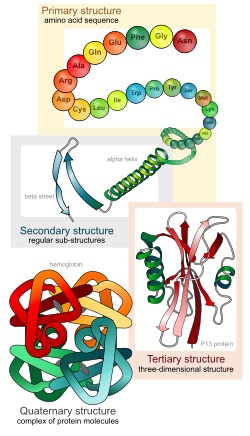
\includegraphics[scale=0.85]{../figures/protein_structure_levels_en.png} % Figure was taking from...

	\caption[Hierarchical distribution of layers in protein structure.]{Hierarchical distribution of layers in protein structure. Image Credit: Mariana Ruiz Villarreal (\url{https://commons.wikimedia.org/wiki/File:Main_protein_structure_levels_en.svg})}
	\label{fig:hierarchy_figure}
\end{figure}
\par The traditional paradigm of protein structure has been challenged by some exceptions of proteins lacking of a fixed or ordered 3D structure. The intrinsically disordered proteins (IDPs) cover a wide spectrum of states from fully unstructured to partially structured including conformations such as \textit{random coils} or \textit{molten globules}. Moreover, some  factors may lead to the permanent loss of structure of a protein, and when that occurs, they endanger the entire organism. How problematic protein misfolding can be for the organism is illustrated by examples such as cystic fibrosis, Alzheimer's, Parkinson's and Huntington's diseases. \\
Chothia and Lesk in the 80s \cite{StructureSequence} helped to set up the fundamentals of what is considered a central paradigm in protein evolution: protein structure is more conserved than sequence (Figure \ref{fig:strucrure_sequence_figure}). However, not all the regions in a protein structure are equally conserved. It has been shown that functionally important amino acids, responsible of the interaction with other molecules, are more conserved than the rest of the protein structure \cite{conservPPI}. Additionally, the structural core is more conserved than the surface \cite{Raj2007}. The high degree of conservation of the protein core enables the protein to maintain the global shape, while the surface is free to change \cite{Todd2001}. These evolutionary mechanisms are in accordance with the central \textit{sequence $\rightarrow$ structure $\rightarrow$ function} paradigm that prevails in the protein evolution field. 

\begin{figure}[htbp]

  \centering
  	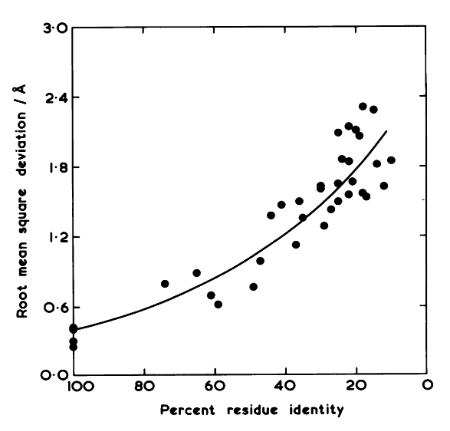
\includegraphics[scale=0.5]{../figures/structure_vs_sequence.png} % Figure was taking from...

	\caption[Relationship between the residue sequence identity and the structural similarity]{The original plot of the relation of residue identity and the RMSD deviation of the backbone atoms of the common cores of 32 pairs of homologous proteins. Figure extracted from \cite{StructureSequence}}
	\label{fig:strucrure_sequence_figure}
\end{figure}
 
\subsubsection{Protein Structure Determination}\label{structure determination}

\par Since 1960, when the Brithis biochemist John Kendrew determined the myoglobin structure \cite{KENDREW1960}, more than 37,000 different protein structures have been deposited in the Protein Data Bank (PDB) \cite{Berman2000}. The PDB is a repository created in the 1970s with the aim of storing all the 3D protein structures and unifying their format. Figure \ref{fig:structures_pdb} shows the variation of the number of deposited structures over the time. The number of PDB structures has significantly increased over the last years thanks to initiatives such as the Protein Structure Initiative (PSI) \cite{Norvell2007} or the Structural Genomics Consortium \cite{GIleadi2007}. The later, was born with the aim of determining the structure of all human proteins. However, soon after, they realized that the goal was unrealistic. Fortunately, the number of folds which represent the complete \textit{fold space} observed in nature is much smaller that the number of proteins. Therefore, the current goal is to determine the structure of a representative set of proteins, that is, at least one protein per fold class. Subsequently, using the structure of representative proteins as templates, and thanks to the \textit{homology modeling} techniques (\cref{Homology_modeling}), it is usually possible to infer the structure of other proteins belonging to the same fold class as we will explore further in the next \cref{structure_predicion}.

\begin{figure}[htbp]
  
  \centering
    \begin{subfigure}[b]{0.75\textwidth}
	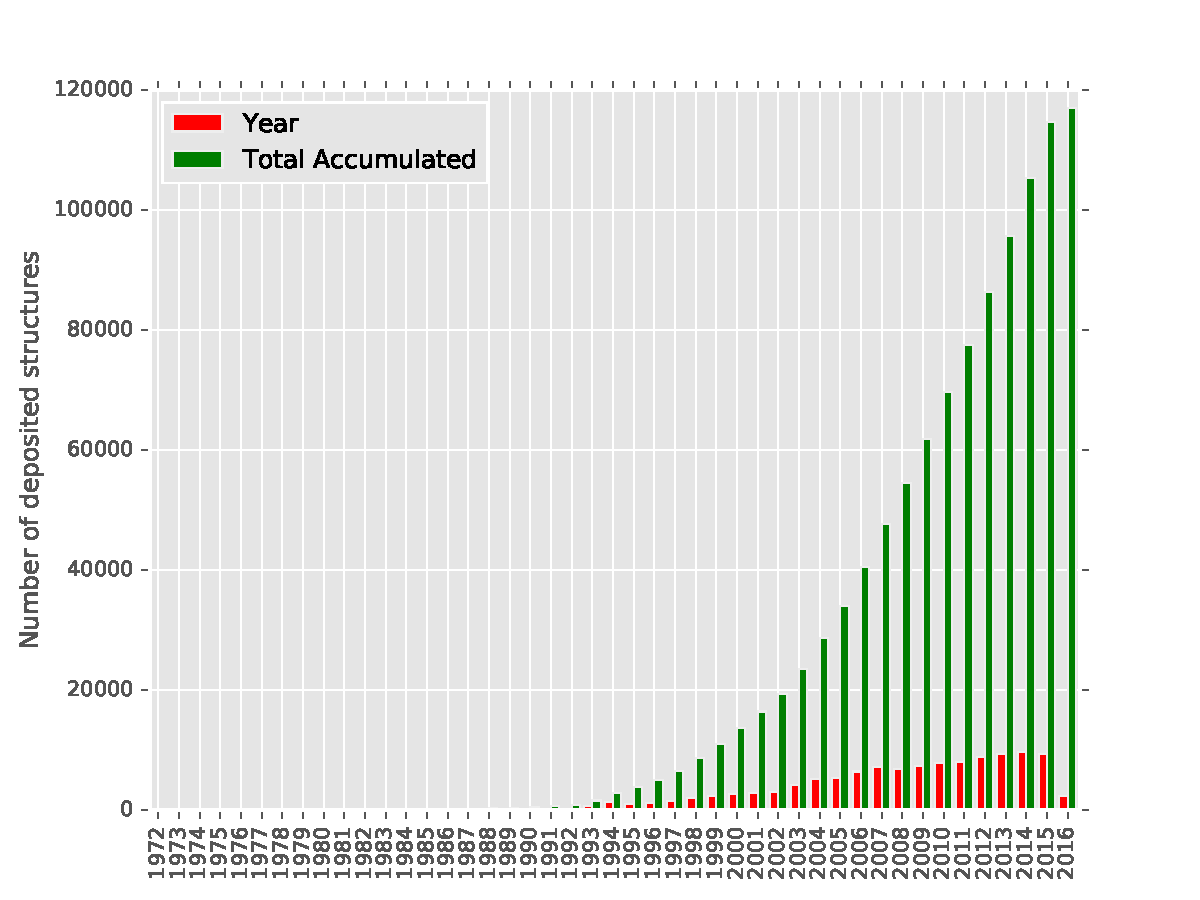
\includegraphics[width=1\linewidth]{../figures/pdbs_per_year.pdf}
	\caption{}
	\label{fig:structures_pdb}
	\end{subfigure}
	\begin{subfigure}[b]{0.75\textwidth}
	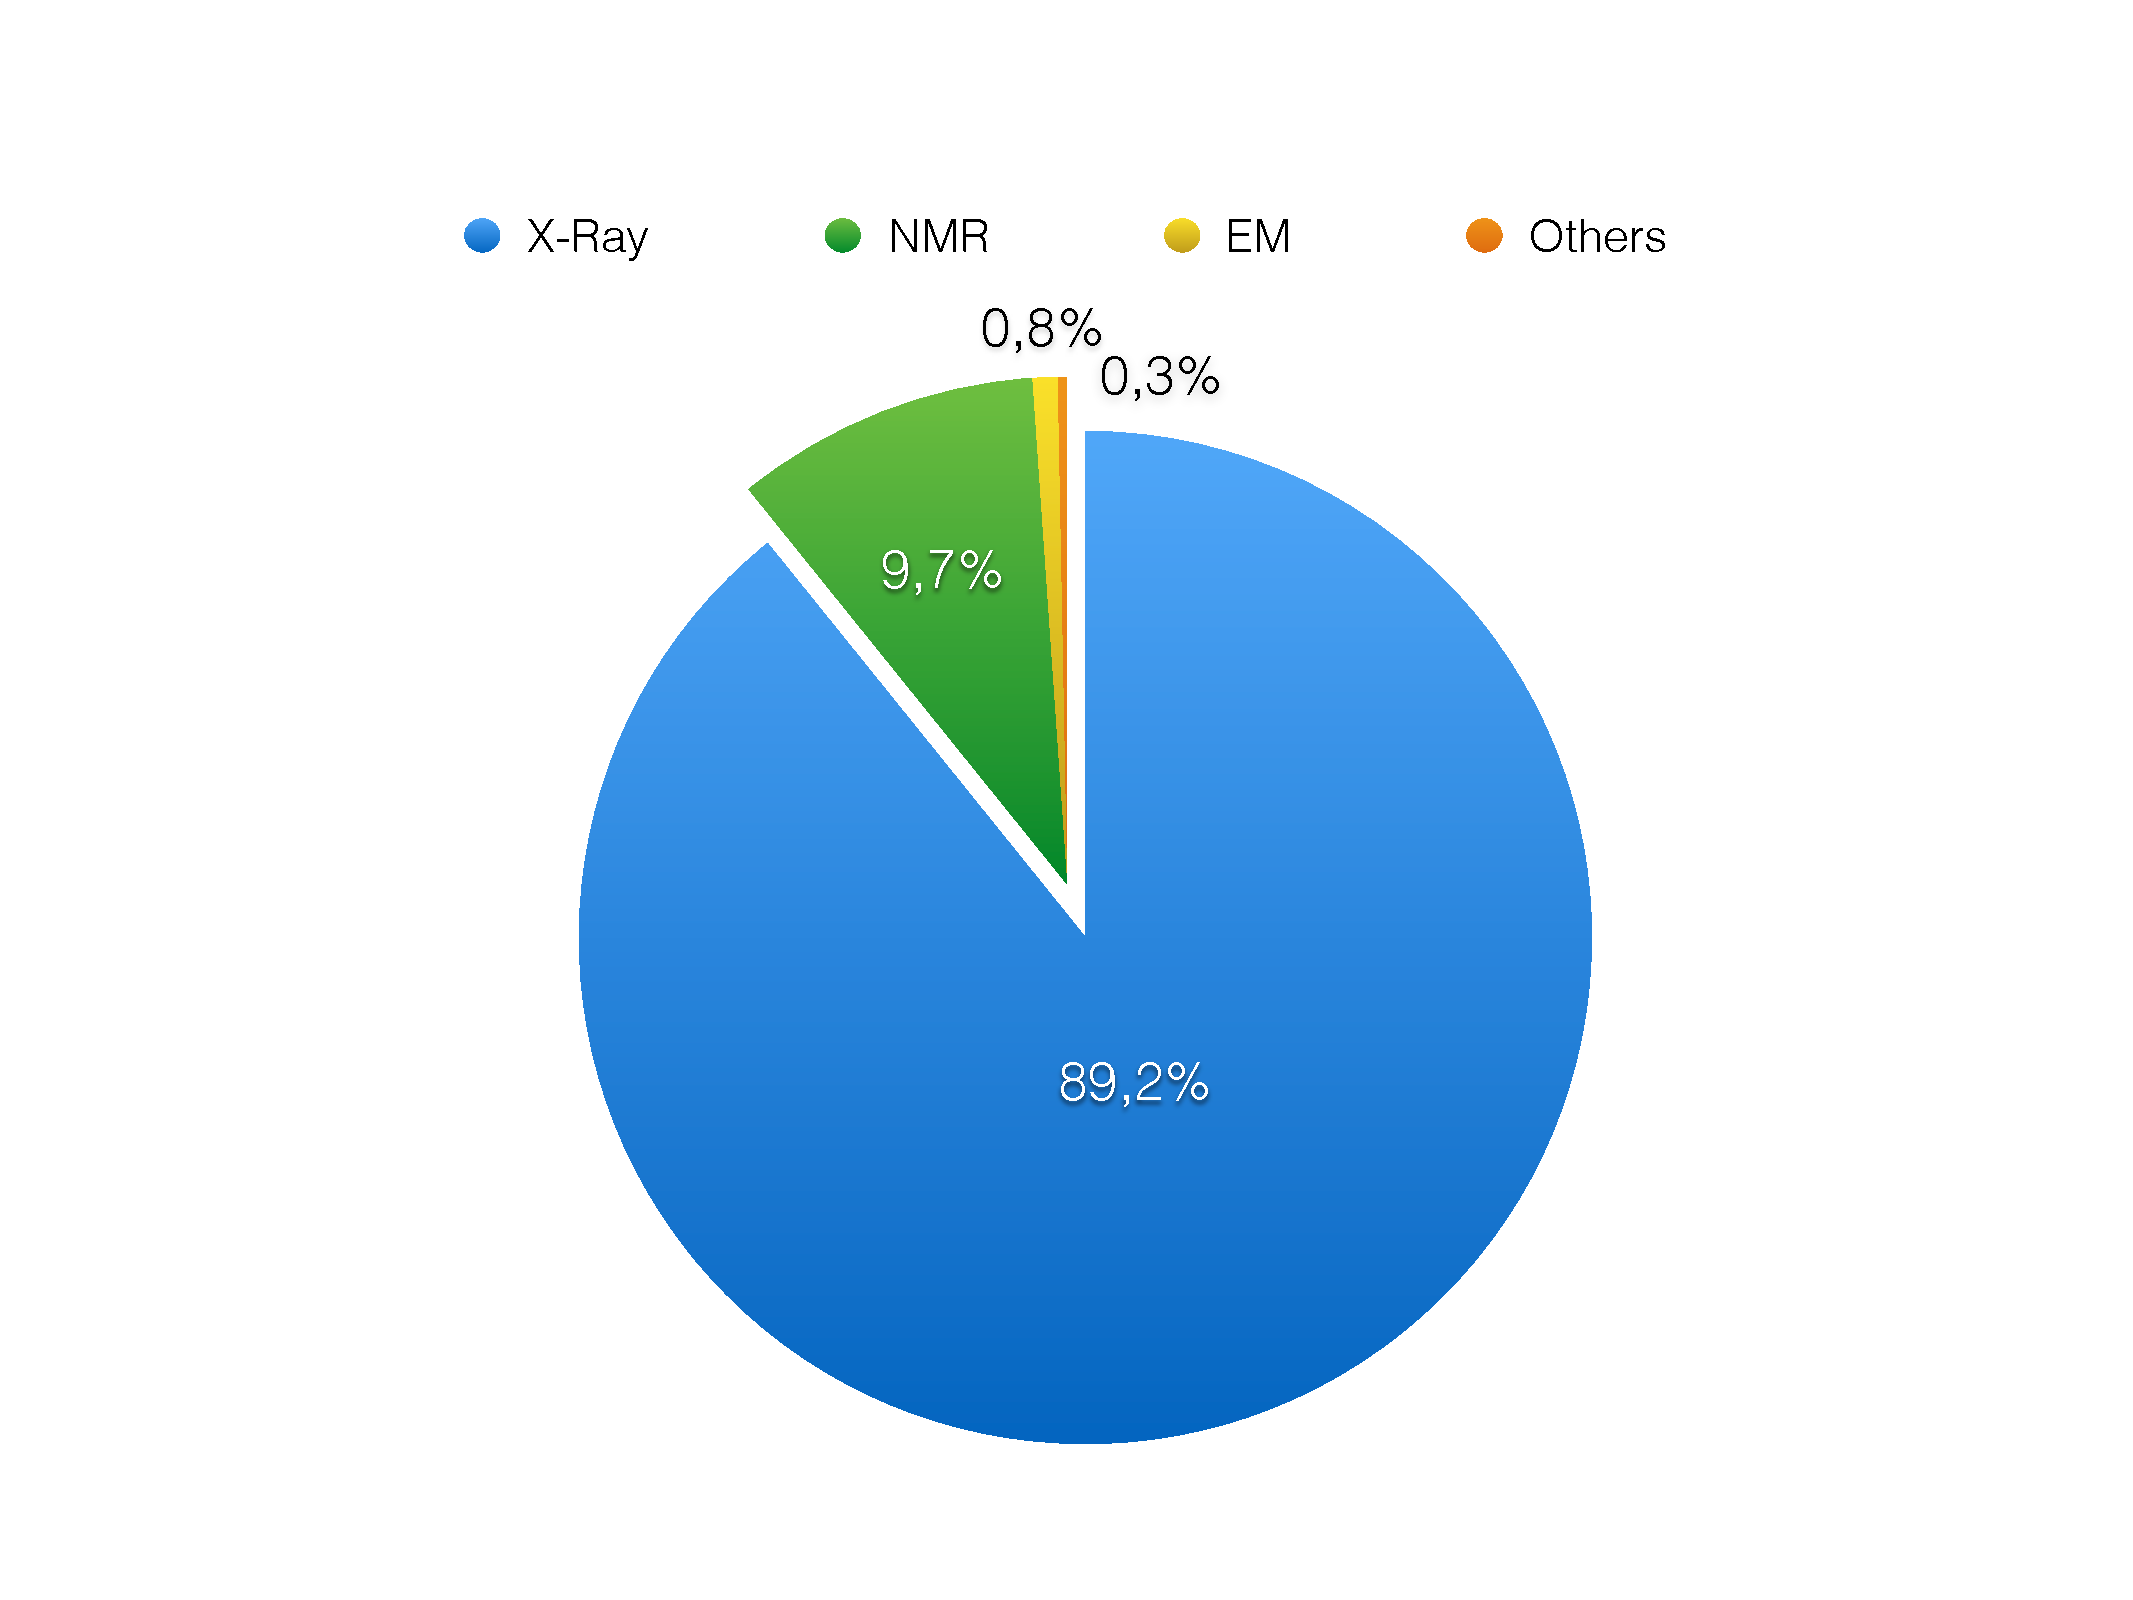
\includegraphics[width=1\linewidth]{../figures/pie_smethods.pdf}
	\caption{}
	\label{fig:smethods_pie}
	\end{subfigure}
   \caption[Deposited structures in PDB per year]{a) Growth of released structures per year. Data extracted from PDB. b) Pie chart with the percetange of structures determined by the different methods. Data extracted from PDB.}
   
	
	
\end{figure}
 

\par Several methods are currently used to experimentally determine the 3D structure of a protein. More than 99$\%$ of structures deposited in the PDB have been determined by the three main methods:  X-ray crystallography (X-ray), nuclear magnetic resonance  spectroscopy (NMR) and electron microscopy (EM) (Figure \ref{fig:smethods_pie}). These methods provide experimental data that helps scientist to elucidate the final structure of a protein. However, in most cases, the experimental data is not sufficient by itself to build an atomic model. Additional knowledge about the molecular structure most be added. For example, the preferred geometry of atoms in a standard protein, the patterns of repulsion and attraction of amino acids, etc. All this information allows the building of the final model that is consistent with both the experimental data and the prior knowledge of the 3D geometry of the molecules. I next briefly explain the three aforementioned methods:

\begin{enumerate}[label=(\alph*)]
\item \textbf{X-ray crystallography}. Currently, it is the most widely used method in protein structure determination. Almost 90$\%$ of the structures deposited in PDB come from X-ray crystallization (Figure \ref{fig:smethods_pie}). In this method, X-rays fired at a crystal of the molecule are diffracted by the electron clouds of the protein atoms, forming an unique pattern that is printed as a picture of the atomic density map. Subsequently, the diffraction pattern is combined with other physio-chemical knowledge of the protein, such as composition or atomic geometrical restrictions, in order to build the final 3D model \cite{Smyth2000}. 
\par Before the X-ray exposition, it is then necessary a prior step of crystallization of the molecule.  Unfortunately, the crystallization step introduces several limitations.  The flexibility of proteins is one of the these limitations. The flexible nature of proteins makes really difficult the creation of an accurate and homogeneous alignment of multiple molecules used to create the crystal. Another important limitation is the different conditions required for crystallizing each different molecule. These limitation are especially noteworthy in membrane proteins. Despite of nearly 30$\%$ of eukaryotic proteins are membrane proteins, only 604 unique membrane protein structures have been solved to date (data extracted from \url{http://blanco.biomol.uci.edu/mpstruc/}, March 2016). Therefore, alternative innovative techniques are needed to overcome the numerous obstacles associated with X-ray structure determination of membrane proteins \cite{Bill2011}. 
\par The accuracy of the final atomic structure relies on the quality of the generated crystals. Two important measures of the accuracy of a crystallographic structure are the \textit{atomic resolution}, which refers to the smallest separation between crystal lattice planes that is resolved in the diffraction pattern \cite{Yaffe2005}, and the \textit{R-factor}, which measures how well the refined structure predicts the observed data \cite{Morris1992}. 

\item \textbf{NMR spectroscopy}. The NMR spectroscopy technique has been used for years to determine the structure of proteins. Currently, almost 10$\%$ of the structures deposited in PDB have been determined by this method (Figure \ref{fig:smethods_pie}). In NMR spectroscopy, the protein is purified, placed in a strong magnetic field, and eventually probed with radio waves. The observed set of atomic resonances is then analyzed to retrieve a list of atomic nuclei that are close in the space. Similarly to X-ray crystallography, this set of restraints is subsequently used to build the structural model of the protein that contains the 3D conformation of each atom in the space \cite{Wider2000}.
\par NMR spectroscopy has a major advantage over X-ray crystallography: it provides information on proteins in solution. Therefore, this method is the main method for studying the atomic structure of highly flexible proteins. A standard NMR structure includes an ensemble of protein structures, all of them being consistent with the experimentally observed set of restraints. The ensemble of structures are very similar in those regions with strong restrains, less constrained regions of the proteins, on the other hand, show less agreement in the generated models. These lack of restriction areas are presumably the flexible regions of the protein since they do not provide a strong signal in the experiment. 
\par A limitation in comparison with X-ray crystallography is its applicability, this technique is usually limited to proteins smaller than 35 kDa. Moreover, NMR can only be applied to soluble proteins that do not aggregate and are stable during the NMR experiment. NMR is also inherently insensitive and milligram amount of proteins are required \cite{Wider2000}. 
\item \textbf{Electron microscopy (EM)} methods. EM methods are emerging as a very versatile tool for determining the structure of large macromolecular complexes. To date, less than 1$\%$ of proteins in PDB have been determined by EM methods (Figure \ref{fig:smethods_pie}). However, in recent years there has been dramatic increase in the number of complexes determined by EM technologies. The revolution in the structural biology field is perfectly manifested by the cryo-electron microscopy (cryoEM) method: in 2015 alone, cryoEM was used to map the structures of more than 100 different molecules \cite{CryoEM}. In cryoEM a beam of electrons is fired at a frozen protein solution. The
emerging scattered electrons pass through a lens to create a magnified image on the detector, and the structure can then be deduced afterwards. \\
The utility of cryoEM and others EM tools lies on the fact that it allows the observation of molecules that have not been fixed in any way, showing them in their native environment. This is the opposite of the crystallization step in X-ray crystallography, which many times hampers the success of the whole procedure. CryoEM has traditionally been applied to large molecules such as ribosomes \cite{Khatter2015} or the V-ATPase \cite{Zhao2015}, but it has also shown potential in small membrane proteins \cite{Liao2013} and medically relevant proteins \cite{Bai2015}. \\ 
However, there is a big a room for improvement for EM methods. Despite of recent advances in the resolution, most of the cryoEM structures have lower resolution than the X-ray ones. Furthermore, there are numerous unsolved technical  problems that need to be addressed to make easier its standardization and systematic application.
\end{enumerate}
 



\subsubsection{Protein Structure Prediction} \label{structure_predicion}


\par Despite of the advances in methods for protein structure determination, most of the known proteins lack of deposited structure in the PDB. There are more than 65 billion protein sequences in  UniProtKB (\url{http://www.uniprot.org}, August 2016), including 551,705 manually annotated and reviewed. However, only about 4$\%$ of the later group (\textit{i.e.,} 23,195 different protein sequences) have a link to a PDB structure. Therefore, there is a gap between the number of known protein sequences and the number of determined structures, the so-called \textit{sequence-structure gap} \cite{Rost1996}. Computational methods for structure determination are helping to bridge this gap. The prediction of the 3D structure of a protein from its amino acid sequence has always been one of the most desirable goals in computational biology. It would save a lot of resources, and it would set a milestone in the structural biology field. Unfortunately, we are still far from being able to predict the structure of many proteins from their primary sequence. Overall, four different approaches are commonly used. The first, and most extensively used, is the \textit{homology} or \textit{comparative modeling}, that uses similar experimentally determined structures to model the structure of the protein of interest (\cref{Homology_modeling}). Second, \textit{fold recognition} and \textit{threading} methods are used to model protein structures with low similarity to known protein structures \cite{Jones1992, Bowie1991}. Third, \textit{de novo} or \textit{ab initio} methods make their predictions by combining the principles of physics that rule protein folding, with information derived from known structures but without relying in any type of similarity or evolutionary relationship to known folds \cite{Lee2009}. Finally, the \textit{integrative} or \textit{hybrid} methods combine different computational and/or experimental sources to perform the structure prediction \cite{Russel2012}.   
 
\subsubsection{Homology modeling} \label{Homology_modeling}

\begin{figure}[htbp]

  \centering
  	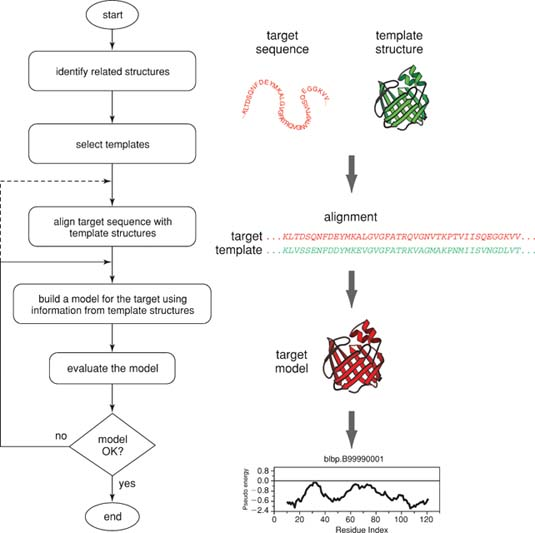
\includegraphics[scale=1]{../figures/workflow.jpg} % Figure was taking from...

	\caption [Workflow in comparative protein structure modeling]{Workflow in comparative protein structure modeling.  The figure has been extracted from \cite{Eswar2007}}
	\label{fig:workflow_modeling}
\end{figure}
\par This type of protein structure prediction method exploits the evolutionary relationship between the \textit{target} protein (i.e., the protein being modeled) and the template(s) with known experimental structure. They are based on the biological premise that evolutionary related sequences tend to have similar 3D structures (\cref{protein_structure} and \ref{structure determination}). Figure \ref{fig:workflow_modeling} shows the regular steps in comparative protein structure modeling: 
\begin{enumerate}
\item \textbf{Identification of suitable template(s) structure(s) similar to the target protein}. This step consists on a search for similar sequences with known 3D structure. This task is easy when the 3D structure of a close homologue of the target protein has been experimentally determined. Initiatives such as the PSI \cite{Norvell2007} are helping to this issue by increasing the number of modellable proteins. However, there are still many proteins lacking of homologous proteins in PDB. In these cases, alternative methods such as \textit{ab initio} modeling might be used.  

\item \textbf{Alignment between the target and the template(s) sequence(s)}. The sequence identity of the target-template alignment is the most frequently used measure for similarity. Consequently, the sequence identity is also a good predictor of the final 3D model quality. The overall accuracy of models calculated from alignments with sequence identity higher than 40$\%$ is usually good (i.e., RMSD \footnote{Root Mean Square Deviation is the measure of the average distance between the atoms of two superimposed proteins. Equation $RMSD=\sqrt[]{\frac{1}{N} \sum\limits_{i=1}^N \delta_i^2}$ where $\delta_i$ is the distance between the $N_i$ pair of equivalent atoms (usually the C$\alpha$).}  lower than 2.0\AA). In the 30$\%$-40$\%$ identity range, errors can be more severe and are often locate in loops and highly flexible regions. Below the 30$\%$ of sequence similarity, often referred to as \textit{twilight region}, serious errors occurs including the basic fold being mispredicted \cite{Baker2001, twilight1996}.
Figure \ref{fig:homology_modeling} shows an empirical threshold for homology modeling extracted from \cite{Sander1991}. The region below the curve gathers those cases where the alignment does not carry enough information to model the 3D structure, while area above the threshold curve, include those cases where homology modeling is applicable.  
\begin{figure}[htbp]

  \centering
  	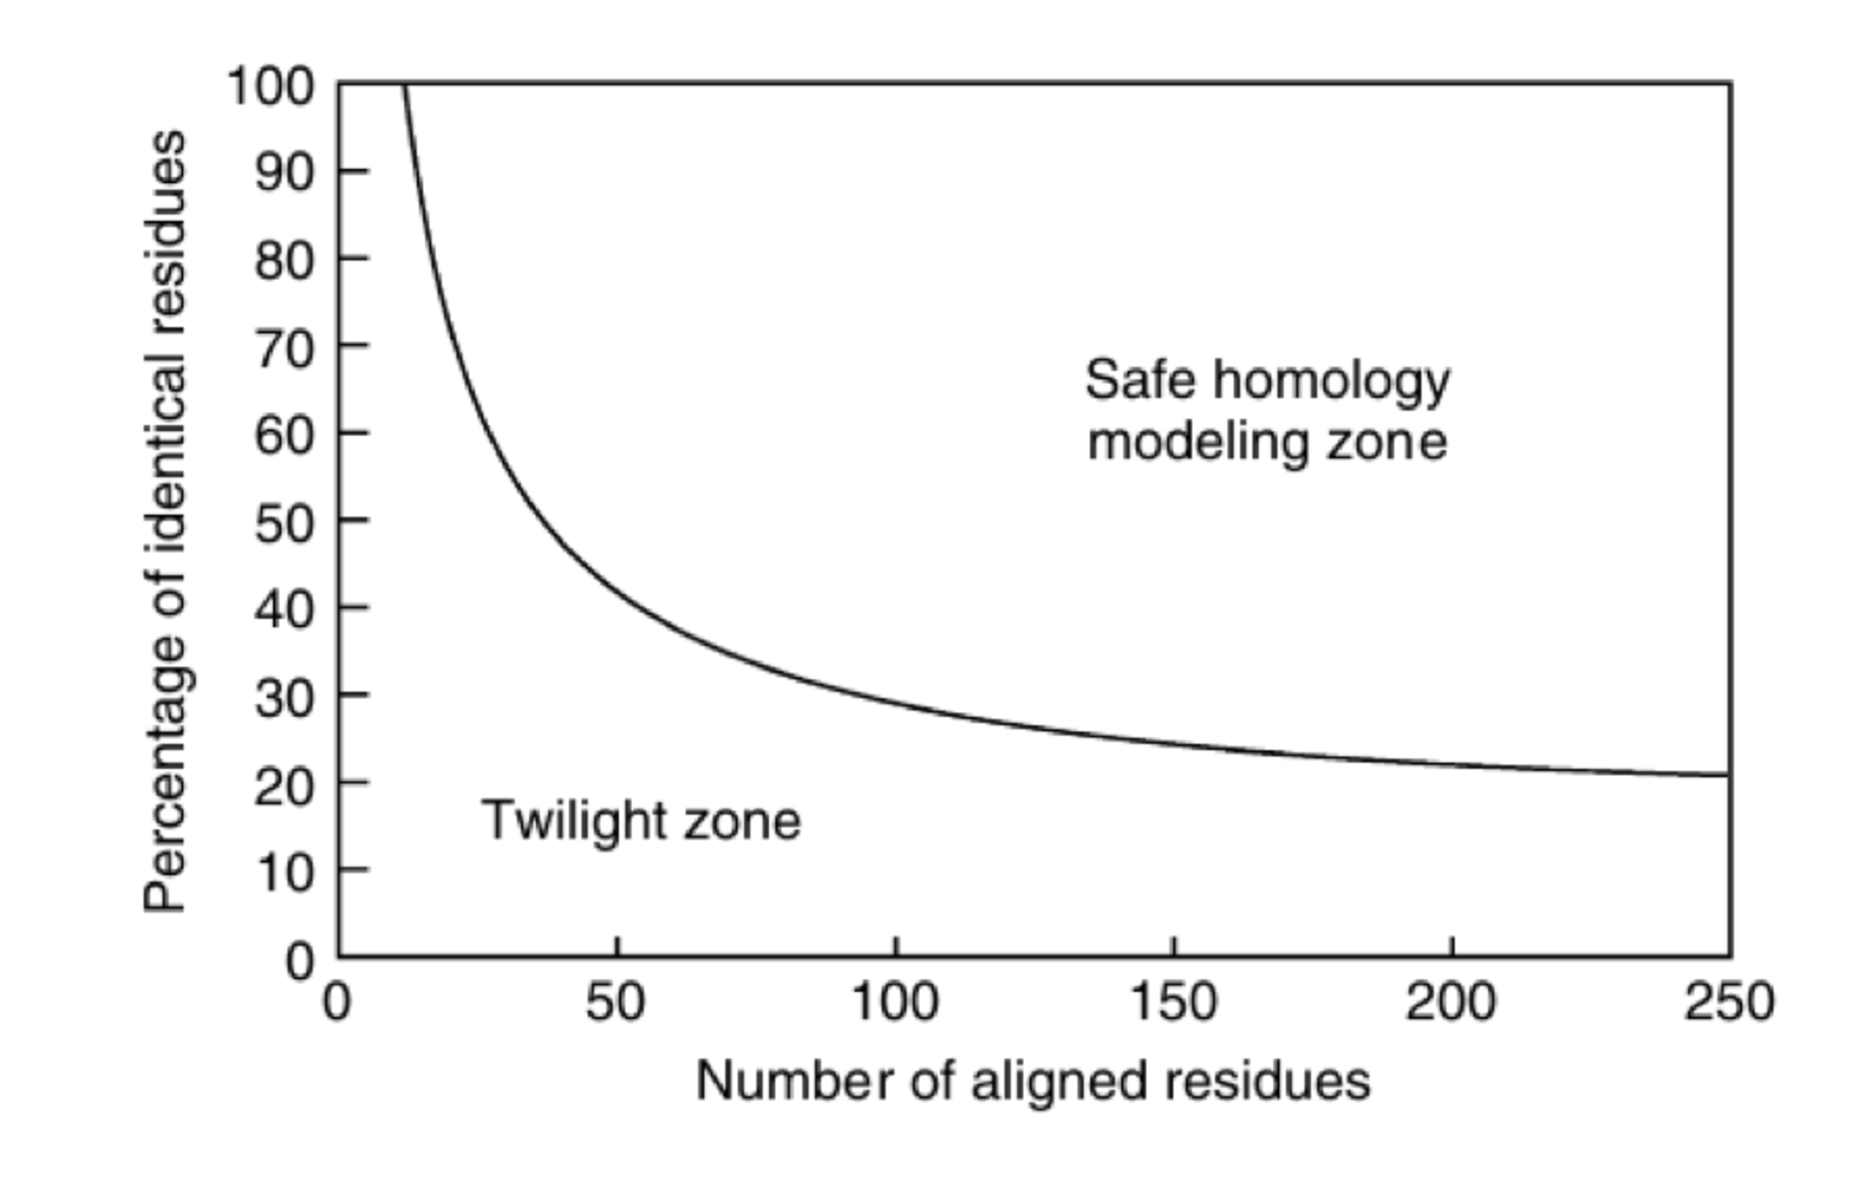
\includegraphics[scale=0.35]{../figures/homology_plot.pdf} % Figure was taking from...

	\caption[Homology threshold curve as a function of alignment length]{Homology threshold curve as a function of alignment length. Data extracted from \cite{Sander1991}}
	\label{fig:homology_modeling}
\end{figure}
\item \textbf{Modeling and refinement of the structurally conserved regions and prediction of the structurally variable regions.} There are different algorithms to assign the spatial coordinates of the target protein using the template(s)-target alignment information. Highly conserved regions are generally well modeled, while those regions with insertions or gaps are more prone to include errors and suboptimal atomic orientations. Next, the model is refined to idealize bond geometry and to remove errors that may have been introduced in the modeling step. The refinement process pursues the free energy minimization of the generated 3D protein model. Many different algorithms have been applied to perform the minimization step, including molecular mechanics force fields \cite{PRO1410}, molecular dynamics \cite{Fiser2000}, Monte Carlo simulations  \cite{Kidera1995} or genetic algorithms \cite{McGarrah1993}.
 
\item \textbf{Evaluation of the model(s).} Model evaluation seeks for the identification of the different errors that might have occurred during the modeling process. Multiple methods have been developed to assess the quality of a 3D model. In fact, 3D model assessment was included from the seventh edition of the CASP experiment \cite{PROT21669}. The general question of how accurate is a model can be reformulated in several specific questions: 



\begin{enumerate}[label=\roman*]
\item \textit{Is the selected fold correct?} The fold assessment consist of deciding whether a given protein model has the right fold. Residue-based combined accessible surface and distance-dependent scoring functions have shown the best performance in this task \cite{Melo2002}. 
\item \textit{How do we select the best model among the set of decoys or alternative solutions?} Several models can be generated by making changes in the template-target alignment, by selecting different template(s) structure(s) or by using different seeds in the refinement non-deterministic algorithms. Atom-based distance-depend scoring functions have proved to be useful for this particular task in some cases \cite{Samudrala1998}. However, there is not a gold standard for ranking the generated 3D models. Thus, the model selection eventually relies on the expertise of the person running the experiment. 
\item \textit{Which is the overall accuracy of the model? Which is the accuracy of the model in a particular region of the model?} These questions can be addressed by defining scores that correlate with the RMSD after superimposing a model and its native structure. Numerous scoring functions have been implemented to address this issue. The physics-based scoring functions attempt  to  approximately  calculate the  atomic  interaction  energies  in  the  system. These scoring functions usually encode a set of parameters that describes the energy of a system of particles. Examples of these scoring functions are AMBER \cite{CASE2005}, CHARMM \cite{Brooks1983} or MM-PDBSA \cite{Fogolari2003}. Differently, the knowledge-based potentials or potentials of mean force, are scoring functions derived from an analysis of empirical information. The physical meaning of potentials of mean force has been widely disputed since their introduction \cite{Thomas1996}. Nevertheless, since they frequently correlate with the actual free energy differences, they have been broadly used with significant success \cite{Shen2006, Zhou2002, Sippl1995}. 
\end{enumerate}
\end{enumerate}

\par The application of comparative modeling is limited by several aspects. First, is the availability of a suitable template. Despite of the efforts made to determine at least one structure per known fold \cite{Norvell2007}, divergences between the template and the target hampers the modeling of a correct 3D structure. In fact, models based on alignments with sequence identity below 30$\%$ may be unsatisfactory (Figure \ref{fig:homology_modeling}). The lack of template problem is even more noticeable in membrane proteins. The limited number of membrane proteins with 3D experimentally determined structure available makes their modeling an extremely difficult task. However, the high value of these proteins in diverse therapeutic areas \cite{Du2012, Kampen2011} is fostering the development of specific membrane protein modeling methods \cite{Leman2015}. Another aspect restricting the success of homology modeling is the innate flexibility of proteins. Highly flexible regions are more difficult to model and consequently are more prone to errors than more rigid parts of the structure. Despite of these limitations, homology modeling has been successfully applied to many proteins and its currently the main approach to computationally model the 3D structure of proteins\footnote{For a comprehensive review of homology modeling methods, applications and limitations please consider \cite{Marti-Renom2000, Malmstrom2010}}. 
\par There are many computational methods to predict the 3D structure of proteins (Table \ref{table:table_software}). Each of these methods have their own strengths and weakness and none of them clearly outperforms the others for all cases.
 
\renewcommand{\arraystretch}{1.2} %<- modify value to suit your needs

\begin{table}[h!]
 \centering
 \begin{adjustbox}{width=1\textwidth}
 \begin{tabular}{||c | c |c||} 
 \hline
 \tr\textbf{Modeling Tool}\br & \tr\textbf{Website}\br & \tr\textbf{Reference(s)}\br\\  
 \hline
 Modeller & \url{https://salilab.org/modeller/} & \cite{Eswar2007, Sali1993}  \\ 
 \hline
 SwissModel & \url{http://swissmodel.expasy.org} & \cite{Biasini2014} \\
 \hline
 HHPred & \url{http://toolkit.tuebingen.mpg.de/hhpred} & \cite{Soding2005}  \\
 \hline
 I-Tasser & \url{http://zhanglab.ccmb.med.umich.edu/I-TASSER/} & \cite{Yang2015a, Roy2010, Zhang2008}  \\
 \hline
 Rosetta & \url{http://robetta.bakerlab.org/} & \cite{Kim2004}   \\ 
 \hline
 RaptorX & \url{http://raptorx.uchicago.edu/} & \cite{Kallberg2014} \\
 \hline
 3DJIGSAW & \url{http://bmm.crick.ac.uk/~3djigsaw} & \cite{Bates2001} \\
 \hline 
  WhatIf & \url{http://swift.cmbi.ru.nl/whatif/} & \cite{Vriend1990} \\
   \hline
\end{tabular}
\end{adjustbox}

\caption[Examples of public protein modeling tools]{Examples of public protein modeling tools alongside their website and original references.}
\label{table:table_software}
\end{table}




\subsubsection{Protein function}

\par One of the main questions in the protein biology field is to understand the protein sequence-structure-function relationship. It is known the structure of a protein determines its biological function. However, different regions of the structure can perform semi-independent functions from each other. These regions are referred to as protein domains. A domain is a substructure produced by any part of the polypeptide chain, which folds independently into a compact and stable structure \cite{Richardson1981, Bork1991, DomainDef}. Domains on average range 80-250 residues \cite{Islam1995}. Estimates of the number of domains per protein say that more than 70\% of procaryotik proteins and 80\% of eukaryotic proteins include more than one domain \cite{Han2007, Chothia2003}. Among this multi-domain proteins, 95\% of them contain two to five protein domains \cite{Han2007}.  Domains are not only the basic functional units of proteins but also their evolutionary units. As proteins have evolved, domains have been modified and combined to build new proteins \cite{Vogel2004, Apic2001}. 
Such is the importance  of domains in protein evolution, that they have been included in current protein classification methods as one of the major classification parameters. Some of these domain classification methods such as SCOP \cite{Murzin1995} or CATH \cite{Orengo1997} are purely based on the structure, while others such as Pfam \cite{Bateman2002} or INTERPRO \cite{Hunter2009} include information about the function in their classification. 
\par Domains, and consequently proteins, perform its biological activity by interacting with other molecules. Proteins can interact with other proteins, constructing a protein-protein complex; with ions or with small-molecules. The substance that is bound to the target protein is called the ligand, while the region of the protein where the ligand is binding is called ligand's \textit{binding site} \footnote{For simplicity, in this thesis, unless otherwise indicated, the term ligand will only refer to small molecules ligands, while proteins ligands will be explicitly named as protein-protein interactions}. The next section is focused on protein-compound interaction presenting the basis for all the work developed during the thesis. 



\subsubsection{Protein-Ligand Interactions} \label{ligand_intect}


\par The roles played by the protein ligands are diverse. Catalysis of enzyme substrates, regulation of the protein activity, cellular communication or defense from external attackers are just few examples of the multiple functions that small-molecule ligands perform in living organisms. All these functions are performed by small-molecules that selectively bind to their target proteins. However, given the vast amount of proteins and small molecule ligands in the cytoplasm, how do the small molecule ligands select their protein targets? There have been several protein-ligand binding theories. In the \textit{Lock and Key theory} \cite{Cramer1994}, Emil Fischer proposed a system where the binding sites of enzymes are rigid and pre-adjusted geometrically to the natural substrate (Figure \ref{fig:lock_and_key_model}). This theory became widely accepted for years. Nevertheless, during subsequent years, evidence started to accumulate suggesting that the binding sites of proteins do not match perfectly their ligands, but rather the binding process triggers some conformational changes in the enzyme. Therefore the obsolete Lock and Key model was replaced by the \textit{Induced fit theory} \cite{Koshland1959}. The induced fit theory proposes that initially enzymes do not perfectly match their substrate geometrically. Rather, the binding process triggers a set of conformational changes in the protein binding site that improves the match (Figure \ref{fig:induced_fit_model}). More recently, another theory called the \textit{Monod-Wyman-Changeux model or MWC model} came up \cite{Monod1965}. This theory contends that proteins are able to shift spontaneously between multiple conformations called \textit{substates} \cite{Kitao1998, Petsko1984}. This model could also explain \textit{allostery}, a phenomenon in which the binding of the molecule to the catalytic site is affected the binding of other ligand to a different site. This theory has undergone some changes and the current accepted theory posits that ligands bind preferentially to one of the conformation sampled spontaneously by the protein, and therefore stabilizes it. It means that, by changing the protein's energy landscape, ligands change a less favorable conformation into the most favorable one. This model does not necessarily refute the induce fit theory since in many cases, the restrains applied by the ligand on the binding site is expected to induce some conformational changes that will further stabilize the interaction \cite{Foote1994, James2003}. 

\begin{figure}[htbp]
  
  \centering
    \begin{subfigure}[b]{0.75\textwidth}
	
\includegraphics[width=1\linewidth]{../figures/lock_key_model.jpg}
	\caption{Fischer's \textit{Lock and Key model}. The protein is represented in green and the ligand in red. The ligand's binding site of the protein matches the ligand perfecltly.}
	\label{fig:lock_and_key_model}
	\vspace*{4mm}
	\end{subfigure}
	\begin{subfigure}[b]{0.75\textwidth}
	
\includegraphics[width=1\linewidth]{../figures/induce_fit_model.jpg}
	\caption{Koshland's \textit{induced fit model}. The protein is represented in green and the ligand in red. The overall shape of the ligand matches the binding site. The ligand bindings causes some conformational changes that improves the interaction.}
	\label{fig:induced_fit_model}
	\vspace*{4mm}
	\end{subfigure}
	\begin{subfigure}[b]{0.75\textwidth}
	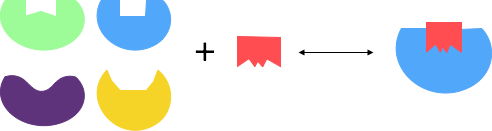
\includegraphics[width=1\linewidth]{../figures/mwc_model.jpg}
	\caption{\textit{MWC model's} representation. The protein changes its conformation constantly (one color per conformation), with at least one these conformation matching the ligand. Its binding triggers some conformational changes that improves the protein's energy landscape.}
	\label{fig:mwc_model}
	\vspace*{4mm}
	\end{subfigure}
   \caption[Schematic representation of the three classic protein-ligand binding theories.]{Schematic representation of the three classic protein-ligand binding theories.}

\end{figure}
\subsubsection{Protein-ligand binding energetics}\label{binding_energetics}

\par The high variety of functions that ligands perform by binding to proteins is also reflected in the diversity of their binding affinity. Binding energies usually range from -2.5kcal/mol to -22kcal/mol \cite{Dunn2001}. The binding strength displayed by proteins matches the biological goal of the binding. For instance, ligands involved in protein communication tend to bind weakly to enable a quick state switch. Cofactors binding to enzymes, on the other hand,  tend to bind strongly to their targets.  The negative sign of the values reflects that is a favorable binding that releases energy: \textit{the binding free energy}.  This energy can be measured experimentally, thorough the equilibrium constant of the binding, or it can be calculated computationally. Formula \ref{equation: Gibbs free energy} and \ref{equation: Kbind} shows, under thermodynamic equilibrium conditions, the relationship between the Gibbs free energy or binding affinity and the equilibrium constant of the binding. $R$ represents the ideal gas constant, $T$ is the temperature, $[C]$ the complex concentration and $[P]$ and $[L]$ the protein and ligand concentration respectively. 
\begin{equation}\label{equation: Gibbs free energy}
\bigtriangleup G=-RTlnK_{bind} 
\end{equation}
\begin{equation}\label{equation: Kbind}
Kbind = \frac{[C]}{[P]*[L]}
\end{equation}
\par These equations show that the binding free energy can be measured experimentally. However, in many cases the experimental measurement are unfeasible or very difficult due to technical problems. Additionally, the expenses associated with these experiments often restricts its broader application. In such cases, computational methods to calculate the free binding energy are needed. The calculation of binding free energy have acquired a remarkable importance in the drug discovery field where the calculation of ligand-target affinity is crucial for pre-clinical phases (\cref{drug_discovery}). Unfortunately, calculation of the ligand-target binding affinity is a extremely challenging task. The main points that should be addressed to accurately calculate the binding free energy are: 
\begin{enumerate}
\item \textbf{The free energy of binding (Formula \ref{equation: Gibbs free energy}) is the difference of two large energies}. The energy of the complex ($E_{pl}$) and the energy of the unbound partners ($E_{p} + E_{l}$) (Formula \ref{equation:energy_complex}): 
\begin{equation}\label{equation:energy_complex}
\bigtriangleup G_bind=E_pl - (E_{p} + E_{l}) 
\end{equation}
\item \textbf{There are two opposite and complex energies driving the process}. The binding enthalpy ($\bigtriangleup H_{bind}$) and the loss of entropy of both the ligand and the protein ($\bigtriangleup S_{bind}$): 
\begin{equation}\label{equation:energy_enthalpy_entropy}
\bigtriangleup G_bind= \bigtriangleup H_{bind} -  T\bigtriangleup S_{bind} 
\end{equation}

\item \textbf{Non explicit representation of the energetic interactions of the system}. Small molecule binding events on a protein cavity implies the displacement of solvent molecules (i.e., usually water molecules). The energy generated by the this exclusion of water molecules is the main driving force in ligand-protein binding \cite{Michel2009a}. Unfortunately, explicit representation and simulation of all the forces involved this event is computationally very expensive. A popular approach to model is to use implicit solvent force fields \cite{Ravindranathan2011, Michel2006, Liu2009}, where the water molecules are represented as a continuous medium instead of individual explicit molecules. The implicit solvation model is justified in liquids, where the potential of mean force are applied to approximate the behavior of many highly dynamic solvent molecules. However, there could be other medias with specific solvation or dielectric properties that are continuous, but not necessarily uniform, since their properties can be described by different analytic functions \cite{Lu2007}. Among the most famous implicit models we can find those based on the Poisson-Boltzmann theory (PB) \cite{Sharp1990} and those based on the Generalized-Born (GB) approximation \cite{Bashford2000}. 
\par Hydrogen bonds and salt bridges between the ligand and the protein can also be a source of free energy gain upon ligand binding. This energy gain comes from the displacement of water molecules bound to the protein. The net gain of energy upon hydrogen bond is around 1-2 kcal/mol. Some scoring functions treat all hydrogen bonds equally, while others, distinguish between neutral and charged ones. Other energies that could be modeled and that contribute to the binding affinity calculations are those generated by interactions with metal ions \cite{Friesner2004}. However, because there may be a covalent component in this type of interactions, its overall binding energy contribution is difficult to model. Finally, nonspecific Van Der Waals and hydrophobic interactions are also included in some methods as additional energy contributors to the overall free energy of binding \cite{Steffen2010}. 
\end{enumerate}

\par One of the main applications of binding free energy calculation is predicting whether a ligand is binding a particular protein target. In other words, given the predicted binding free energy determine whether a specific compound targets a specific protein binding site. In the next section we will explore further these and other approaches aiming at protein-compound interaction prediction.  



\subsubsection[Protein-ligand prediction]{Protein-ligand prediction\protect\footnote{In \cref{nannolyze} we present nAnnolyze, a method for protein-ligand interaction prediction. In the introduction of the mentioned manuscript, there is a discussion of the current state-of-the-art methods in protein-ligand interaction prediction. Therefore, this section is focused in explaining the classification, underlying basics, advantages and disadvantages of the different approaches.}}\label{prediction ligand-target}

The importance of ligand-protein interaction prediction is reflected by the large number of available methods that use multiple different approaches \cite{Csermely2013, prathipati2015}. We can distinguish between \textit{free structure} methods (i.e., methods that do not rely on the protein structure to perform its predictions) and \textit{structure-based} methods. \\    
Free structure methods usually use prior knowledge on protein compound interactions, to further extend the interactions to new and unseen compounds. The development of these methods can be split in two phases. The first step consist on the creation of a predictive model that uses collection(s) of protein-compound interactions to learn hidden relationships between compound and their protein targets.  In the second step, these predictive models are used to extrapolate this knowledge to new and unseen compounds (or targets). The extrapolation relies on different measures of compound or protein similarity. Knowledge-based free structure methods have been assisted by the emergence of new \textit{high-thorughpout screening methods} (HTS) that enabled the creation of large computational compound-protein databases such as ChEMBL \cite{Bento2014}, Therapeutic Target Database (TTD) \cite{Zhu2012a}, Binding MOAD \cite{Hu2005}, BindingDB \cite{Liu2007}, PubChem \cite{Kim2016, Wang2014} or ZINC, among others \cite{Irwin2012}. The recent growth of these collections is accordingly improving their accuracy and coverage. Moreover, since they do not rely on protein structure they can be theoretically applied to any protein or to any compound. Nevertheless, free structure methods do not provide detailed information about the ligand-protein relationship. Information such as binding localization, type of interaction (e.g., allosteric, on-target or off-target) or predicted free energy of binding;  that is absolutely essential in the drug discovery process (Figure \ref{fig:type_ligandtarget_methods}). Consequently, free structure methods are mostly employed in early stages of the drug discovery pipeline. 
\begin{figure}[htbp]

  \centering
  	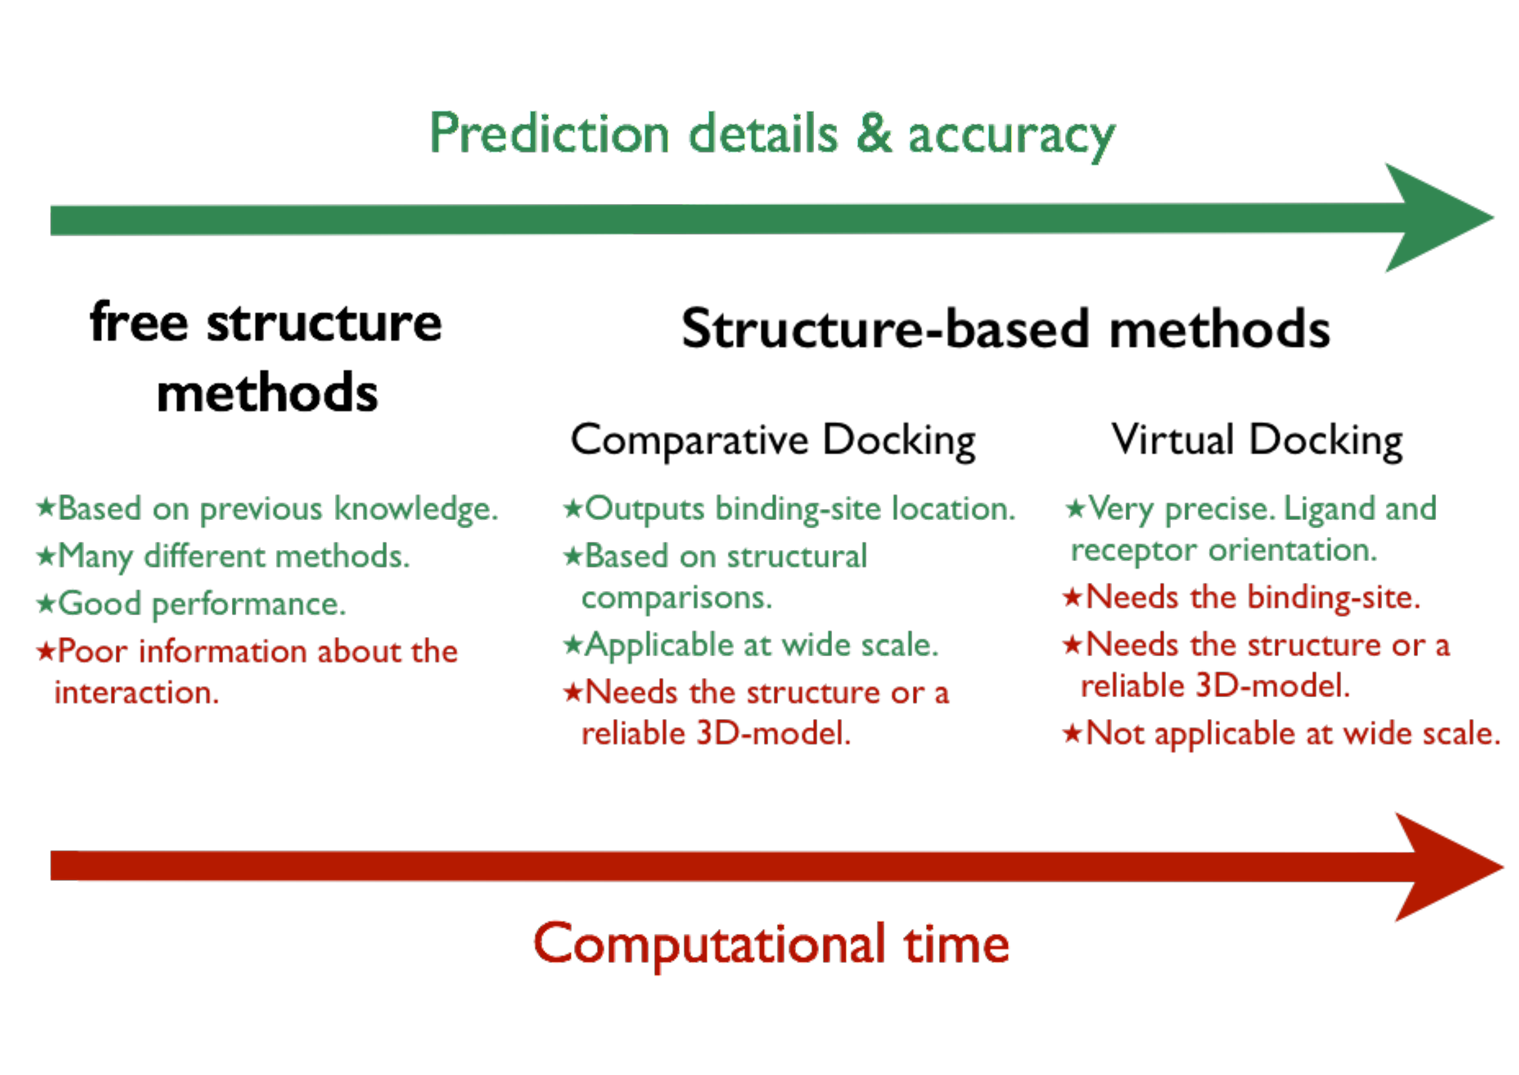
\includegraphics[width=\textwidth]{../figures/type_of_methods.pdf} % Figure was taking from...

	\caption[Type of computational methods for ligand-target interaction prediction]{Classification of the methods for ligand-target interaction prediction alongside their advantages and disadvantages. The red arrow represent the increase in the computational time of the calculus needed for each prediction. The green arrow represents the level of detail of the given output.}
	\label{fig:type_ligandtarget_methods}
\end{figure}
\par Structure based target prediction methods leverage protein's 3D structure to determine whether a small-molecule interact with a protein target. Virtual docking methods have traditionally dominated the structure-based target prediction field. Virtual docking consist on predicting the preferred orientation of one molecule (i.e., the ligand) to a second (i.e., the protein). The process of finding the best orientation of molecule, the so-called binding \textit{pose}, to the protein target is not simple. Several entropic, enthalpic and environmental factors have an impact on the interactions between them (\cref{binding_energetics}). The underlying idea of this approach is to generate a comprehensive set of ligand-protein conformations, and then to rank them accordingly to a specific scoring function \cite{Alonso2006}. The importance of virtual docking methods is not only reflected by the large number of published methods, which include AutoDock \cite{Morris2009, Trott2010}, DOCK \cite{Ewing1997}, FLEXX \cite{Rarey1996}, GOLD \cite{Jones1997} or GLIDE \cite{Friesner2004}, among others; but also by their success in drug discovery applications \cite{Schames2004, Enyedy2001, Vangrevelinghe2003} \footnote{For a comprehensive review of virtual docking methods an applications please consider \cite{Kitchen2004}}. However, virtual docking methods also have some limitations. The most apparent one is that they rely on protein structure. As mentioned above (\cref{structure_predicion}), the coverage of the human structural proteome is below 40$\%$. Thus, some of the most interesting targets in drug discovery lack of experimentally determined 3D structure. In addition to these structurally inherent problems and despite of some massive applications \cite{Reardon2013}, virtual docking methods are still computationally very expensive (Figure \ref{fig:type_ligandtarget_methods}). Additionally, they need the prior knowledge of the binding localization on the protein surface, which many times is unknown before the screening. 

\subsubsection{Comparative docking approach}\label{comparative-docking}

\par To overcome the computational limitations of virtual docking approaches, some structure-based methods use the so-called \textit{comparative docking} approach, which solely relies on structural comparisons, both of compounds and protein targets, to infer new interactions. Comparative docking methods are based on the biological premise that structurally conserved proteins tend to  conserve the biological function \cite{Marti-Renom2007, Laskowski2005, Lee2007, Holm2010}. In other words, structurally similar protein binding sites tend to bind similar ligands. Unlike virtual docking methods, comparative docking approaches do not require the computationally expensive calculations needed to obtain the structural orientation (i.e., the binding pose) of the compound  at the protein binding site. Rather, they provide a more simplistic representation, where the output is usually limited to the binding location on the protein surface, omitting information about the exact binding orientation. Consequently, comparative docking approaches are generally faster and more suitable for large scale virtual screenings than virtual docking methods (Figure \ref{fig:type_ligandtarget_methods}). Several ligand-target interaction prediction methods leverage comparative docking approaches to perform their predictions \cite{Hoffmann2010, Wass2010, Capra2009, Kalinina2011, Marti-Renom2007}. \cref{nannolyze} presents nAnnolyze, a network-based version of Annolyze \cite{Marti-Renom2007}, which is focused on predicting ligand-target interactions at proteome scale. The nAnnolyze chapter further discusses the applications, advantages, disadvantages and limitations of comparative docking approaches in general, and nAnnolyze, in particular.


\subsection{Drug discovery}\label{drug_discovery}

\par Drug discovery is the process by which potential new medications are discovered. It involves a wide range of scientific disciplines, including biology, chemistry, pharmacology and recently also the computational branches of these fields. Historically, drugs were discovered through the identification of the active ingredient from traditional remedies or by serendipitous discovery. Later, the development of synthetic methods allowed the generation of purely synthetic structures that were not found in nature and that were investigated as potential therapeutic agents. More recently, the advent of new genomics, proteomics and HTS techniques, resulted in the identification of large number of novel targets for future drug discovery research. In addition to this \textit{technological revolution}, the advances in bioinformatics and system biology field has prompted the change in drug discovery paradigm towards a more target-centric approach. This modern drug discovery paradigm usually implies the screening of thousands of molecules to identify those that have the desirable therapeutic effect in the previously validated protein target \cite{Drews2000, Patrick2001}. Figure \ref{fig:drug_discovery_pipeline} shows the current drug discovery pipeline alongside the estimated cost and time of each of the phases.  Most modern drug discovery programs begin with the identification of a bio-molecular target whose pharmacological intervention is theoretically beneficial for the treating disease. A target is a broad term that can be applied to a range of biological entities including proteins, DNA and RNA. The target needs to be accessible to the putative drug molecule(s), this property is referred to as \textit{target druggability}. Wrong selection of the target (i.e., weak association between the target and the treating disease) implies lack of the expected efficacy, which is the most important cause of project failure in clinical trials \cite{Hutchinson2011, Lindsay2003}. During the \textit{hit-identification} stage, the target is screened against a set of candidate molecules seeking for the identification of those which able to perform the desired therapeutic activity. Alternatively, in some cases the first step of the discovery process is based on a \textit{Phenotypic screening} of a collection of molecules. This screening pursues the identification of those molecules that perform a predefined function in a biological model. In any case, prior knowledge of the bio-molecular target of the therapeutic activity is generally associated with better outcomes in clinical trials \cite{Hughes2011}. However, there are various drugs in the market with unknown \textit{mechanism of action} (i.e., the drug target remains unknown) \cite{Imming2006}, most of them coming from the traditional drug discovery paradigm. After hit(s){\footnote{ A hit compound could have several definitions. Here we use the one from \cite{Hughes2011}  where they defined a hit as being a compound which  \textit{has  the  desired  activity  in  a  compound  screen  and whose  activity  is  confirmed  upon  retesting.}}   identification, at the \textit{hit-to-lead} stage,  molecular hits are evaluated and undergo limited optimization to identify promising lead compounds for further stages. The optimization to convert a hit to a lead molecule, implies several properties, including the potency, the selectivity and the pharmacokinetics (PK) properties. These lead compounds undergo more extensive optimization in a subsequent step of drug discovery called lead optimization (LO). The main goal of this stage is to maintain favorable properties of lead compound(s) while improving on deficiencies in the lead structure(s). Finally, the selected lead(s) enters into the preclinical stage where the main goals are to determine the safe dose for \textit{First-in-man study} and the first assessment of the product's safety profile. Estimates say that, on average, of every 5,000 to 10,000 compounds that begins the pre-clinical stage, only one becomes an approved drug \cite{Klees1997}. 

\begin{sidewaysfigure}[htbp]
  
  \centering
    
	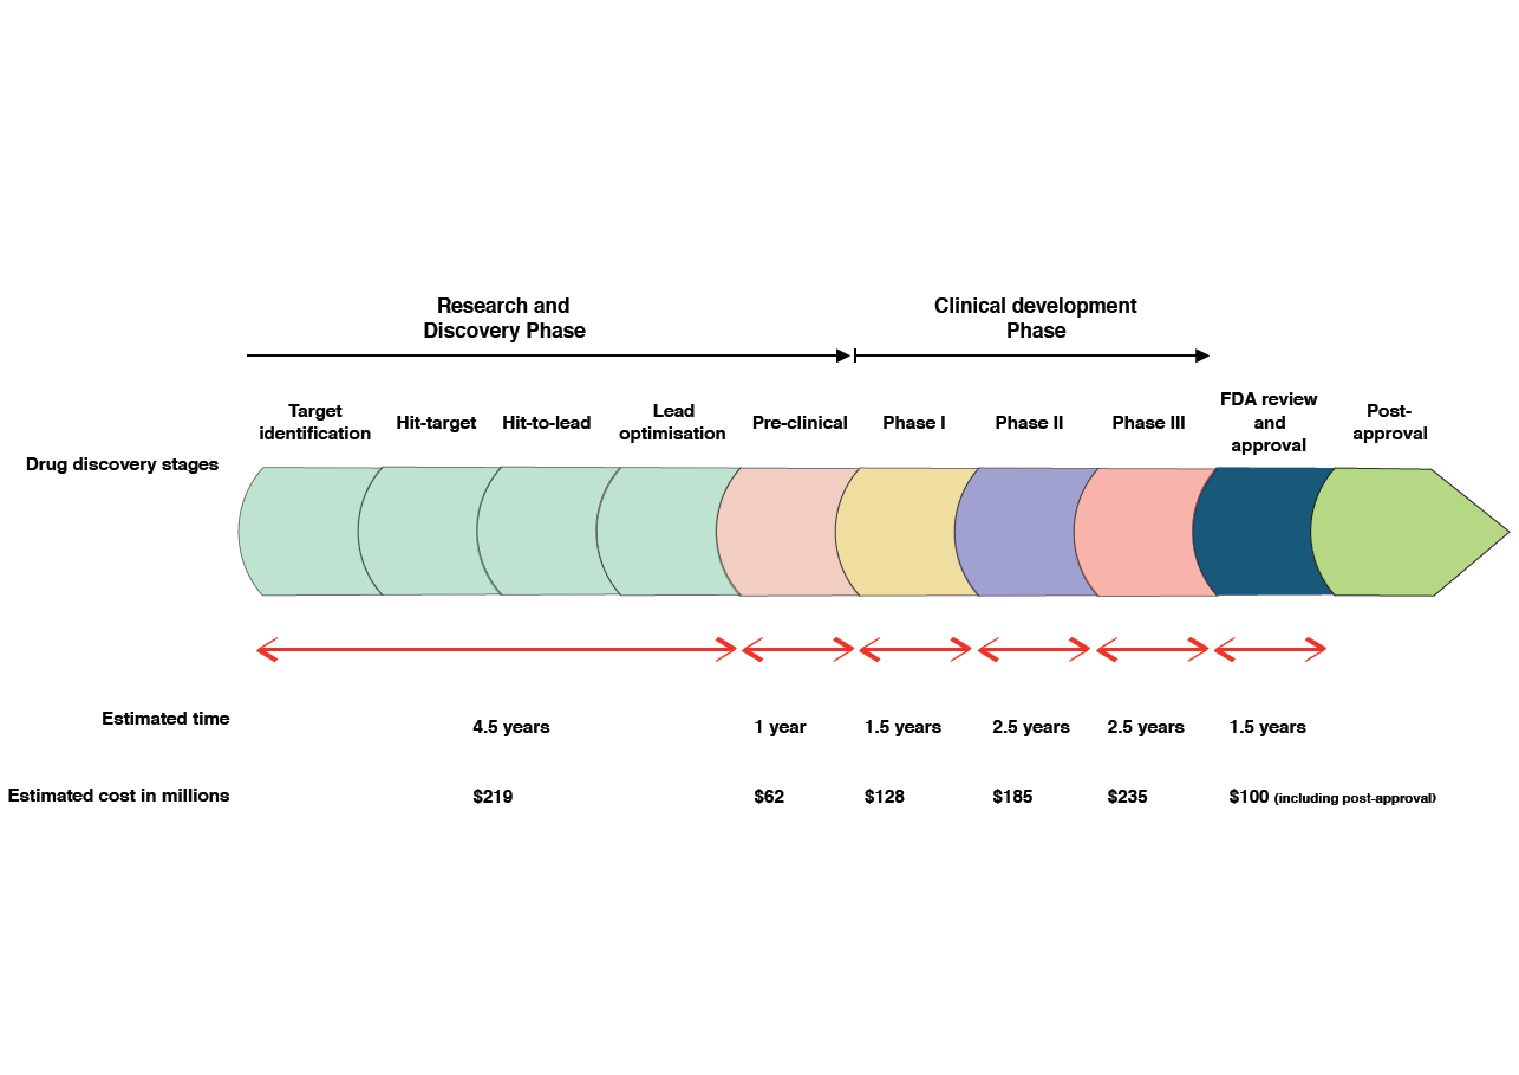
\includegraphics[keepaspectratio=true, width=\textwidth, height=\textheight]{../figures/drug_discovery_phases_3.pdf}
	\caption[Drug discovery and development pipeline]{Drug discovery and development pipeline. For each stage the average cost and time are provided. Post-approval times not included in the time-line. Data extracted from \cite{Paul2010}.}
	\label{fig:drug_discovery_pipeline}
	%\vspace*{4mm}
\end{sidewaysfigure}


\par  According to the The Tufts Center for the Study of Drug Development (\url{http://csdd.tufts.edu}), the development and marketing approval for a New Molecular Entity (NME) takes more than 13 years and around  $\$$2.6 billion (Figure \ref{fig:drug_discovery_pipeline}). In fact, the cost of developing a new drug has dramatically increased since the 1970s (Figure \ref{fig:drug_discovery_evolution}). Currently,  the cost of developing a NME is more than two times the 1990s cost, and more than ten times of the cost of the 1970s.   \\
The raise in the drug development cost has led to a dramatic shrinkage of the efficiency, measured in terms of the number of new approved drugs per billion US dollars of research and discovery (R$\&$D) spending \cite{Scannell2012}. Both research and development phases have significantly raised their expenses (Figure \ref{fig:drug_discovery_evolution}). Factors that have contributed to the raise of clinical costs include increased clinical trial complexity, larger clinical trial size, greater assessment of safety and toxicity drug profiles or evaluation on equivalent drugs to accommodate payer demands for comparative effectiveness data \cite{Scannell2012}. Similarly, factors such as the complexity of the target disease, expenses associated with the application of high-throughput technologies or the complexity of mechanism of action are increasing the prizes of pre-clinical stages. However, pre-clinical associated expenses may be narrowed down with a rational use of the state-of-the-art technologies. In this matter, computational methods are emerging as a tool to speed-up the process by enabling the management of the massive amount of data generated during the discovery stages. Next section introduces different computational methods currently applied during the drug discovery pipeline.  
\begin{figure}[htbp]
\centering
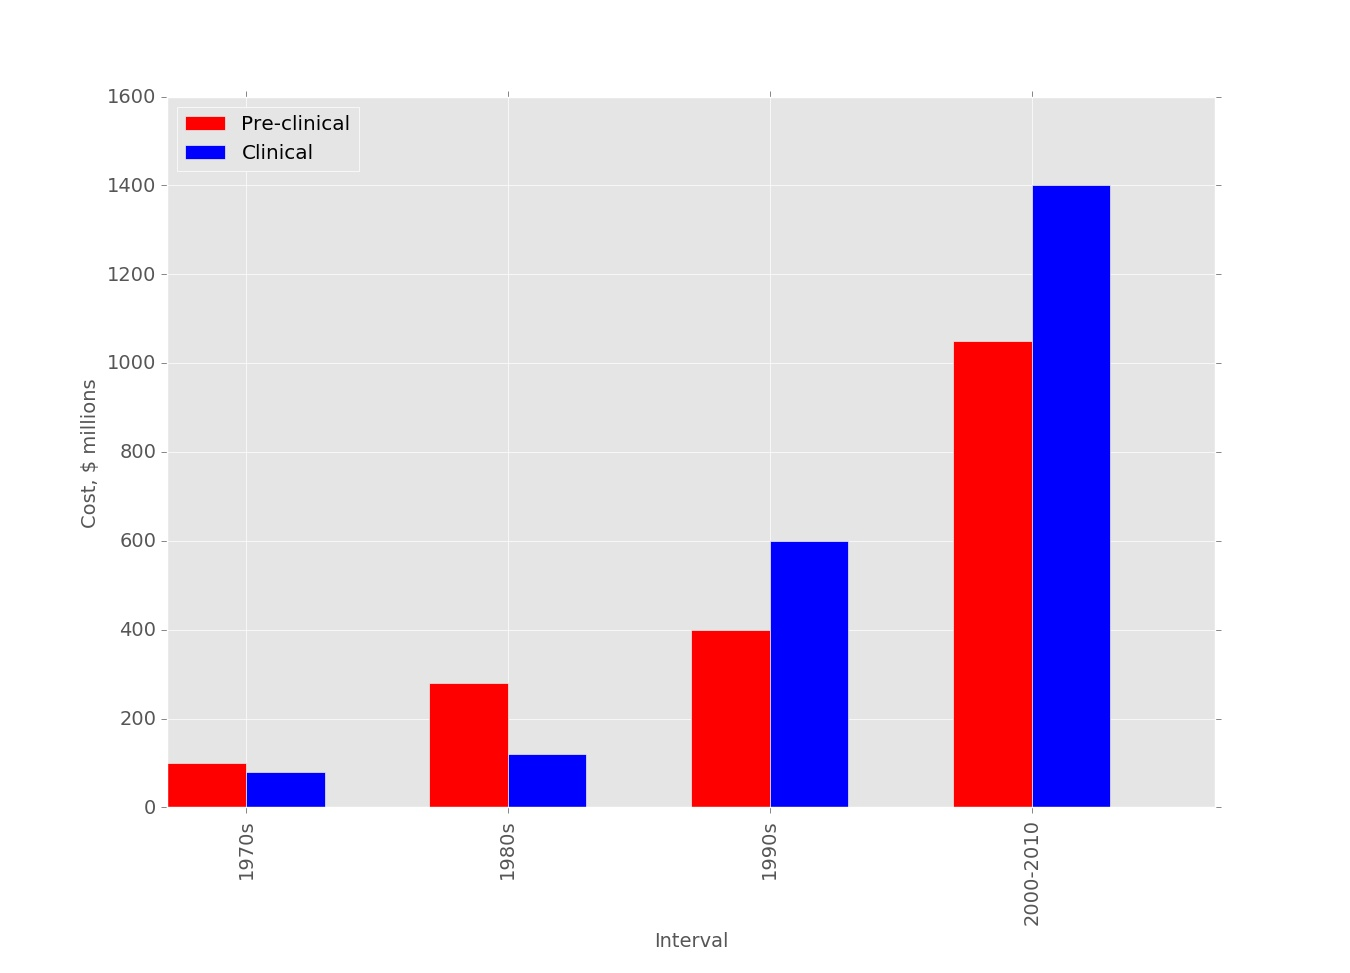
\includegraphics[width=0.9\linewidth]{../figures/drug_discovery_evolution.jpg}
	\caption[Evolution of drug development expenses over time]{Cost of developing a new drug. Blue bars indicate expenses in clinical phases while red represents expenses in pre-clinical stages. Costs are shown in $\$$ millions. Data extracted form: Tufts Center for the Study of Drug Development (\url{http://csdd.tufts.edu/news/complete_story/pr_tufts_csdd_2014_cost_study}).}
\label{fig:drug_discovery_evolution}
	
	\vspace*{4mm}
\end{figure}

\subsubsection{Computational drug discovery}\label{computational drug discovery}

\par Over the last thirthy years, computer-aided drug discovery (CADD) methods, have played a key role in the development of therapeutic drugs \cite{Sliwoski2014}. The modern drug discovery pipeline includes multiple CADD approaches assisting during the drug discovery process:

\begin{enumerate}

\item \textbf{Target identification and validation methods.} Many different computational approaches are used to identify and validate new targets. The \textit{genomics revolution} caused by Next-Generation Sequencing methods (NGS) have significantly increased the development of methods that primary rely on the genetic association between targets and the treating diseases. In some cases, the data is combined with additional information enabling a more precise evaluation of the target viability. Examples of the complementary data include structural data,  
such as experimental structure availability or druggability assessment; system-biology information such as protein-protein interactions, protein pathway analysis or sub-celullar target localization \cite{Yang2009}. Recently, the inclusion of pharmacological data by \textit{drug reporpousing or repositioning} methods has become very popular \cite{Gottlieb2011, Zhang2011, YutakaFukuoka2013}. These methods leverage information of whether the protein is targeted by any FDA approved drug, to prioritize those targets with annotated FDA approved drug(s). Such drug(s) are subsequently applied to the treating disease to validate the target testing hypothesis. Computational methods for target identification and validation have been applied to great variety of diseases, including infectious diseases such as Tuberculosis \cite{Raman2008} or Malaria \cite{Phaiphinit2016}, cancer \cite{Jeon2014} and neurogeneretive diseases \cite{Augustin2012}. 

\item \textbf{Ligand-target prediction}. Once the target has been validated, CADD methods can help in the search of potential target hits. This is one of the fields where CADD methods have been more successful either by making the predictions from scratch or in combination with phenotypic screenings \cite{Martinez-Jimenez2013}. Section \ref{prediction ligand-target} specifies the different methods and their current applications.   

\item \textbf{Quantitative structure-activity relationship (QSAR)}\label{qsar}. QSAR is an approach designed to find relationships between chemical structure and the biological activity of small molecules. QSAR methods are based on the assumption that variations in the biological  activity  of  a  series  of  chemicals  targeting a particular protein are correlated  with variations in their structural, physical, and chemical properties \cite{Perkins2003}. QSAR methods have become an essential tool in the pharmaceutical industry where they play a major role in the hit-to-lead and lead optimization stages. Traditionally, these methods have been used to improve compounds bioactivity. Recently, the applications have been extended to the improvement of ADMET (adsorption, distribution, metabolism, elimination, toxicity) properties \cite{Penzotti2004, Obrezanova2007} and the oral bio-availability \cite{Yoshida2000}. QSAR  methods have undergone rapid changes over the last years. The first 2D-QSAR models were based on descriptors derived from a two-dimensional graph representation of a molecule. These descriptors tried to characterize the most important molecular properties for the molecular interaction. However 2D-QSAR had important limitations for designing new molecules due to the lack of consideration of the 3D structure. Later, 3D-QSAR methods integrated 3D properties of the ligands to predict their biological activity \cite{Verma2010}. The first QSAR model that integrated the 3D geometry to perform the predictions was the Comparative Molecular Field Analysis (CoMFA) \cite{Cramer1988}. In CoMFA, steric and electrostatic features of protein target are mapped onto a surface grid, which envelops a set of compounds superimposed in their active conformation. This grid acts as a surrogate of the binding site of the protein receptor and is frequently referred to as \textit{pharmacophore}. However, this approach has an important limitation: a ligand molecule can only be represented by a single entity. Therefore, if a ligand binds with different conformations, only one of them can be represented in a 3D-QSAR model \cite{Verma2010}. This limitation was overcome by 4D-QSAR methods, which include conformational flexibility and the freedom of alignment by ensemble averaging in the conventional three dimensional descriptors found in 3D-QSAR methods \cite{Hopfinger1997}. 4D-QSAR models have been succesfully applied to simulate binding to cytochrome P450 3A4 \cite{Ekins2000}, HIV-1 protease \cite{Iyer2007} or to the p38-mitogen-activated protein kinase (p38-MAPK), \cite{Romeiro2010} among others \cite{Andrade2010}. More recently, a 5D-QSAR model has been proposed \cite{Vedani2002}. This model includes a new degree of freedom, the fifth dimension, that allows for a multiple representation of the atomic topology of the receptor surrogate (i.e., representation of different induced-fit models of the receptor). Finally, in the 6D-QSAR methods, a greater representation of the different solvation scenarios is included \cite{Vedani2005}. This enables for an even more realistic simulation of the binding process, which is ultimately reflected in the development of better predictive models.   
\item \textbf{Prediction and optimization of the ADMET properties}. Most of the drug discovery initiatives include a computational optimization of the compound's PK properties. As previously mentioned, QSAR methods have been extensively applied to predict the PK properties of compounds. However, there are other \textit{in-silico} approaches that play a substantial role in the ADMET prediction field.   One of the tools that have significantly contributed to the field is the \textit{Lipinski's rule-of-five}, which aims to predict the odds of a compound to become a drug, the so-called \textit{drug-likeness} \cite{Lipinski2004}. The Lipinski's rule-of-five is a rule of thumb created by Christopher A. Lipinski based on the observation of chemical properties of drugs with favorable PK profile. It uses five arbitrary rules based of such number of chemical features to determine whether a compounds is likely to become a drug. If the compound fulfill, at least, four rules then it is considered as a drug-like candidate. However, assessment of compounds drug-likeness in absolute terms does not reflect adequately the whole range of compound qualities. To address this issue, a computational method that quantitatively measures the drug-likeness of a compound has been recently published \cite{Bickerton2012}. Optimization in the ADMET properties of a compound is generally performed during the hit-to-lead and lead-optimization stages, concurrently with the optimization of the compound's bio-activity. This multi-objective optimization process is accomplished in the computational model developed by Besnard and colleagues \cite{Besnard2012b}.\end{enumerate}


\subsection{Drug discovery in Tuberculosis}}

\par About one-third of the world's population is infected with \textit{Mycobacterium tuberculosis} (MTB), the causative agent of tuberculosis (TB) \cite{Lewandowski2015}. Approximately 90$\%$ of infected individuals have latent MTB infections, which remain dormant until activated by specific environmental and host response events. Remarkably, people with compromised immune systems, such as people with HIV, malnutrition or diabetes, or people who use tobacco, have a much higher risk of falling ill. Once the disease has been activated, when left untreated, kills more than half of the infected patients \cite{Connell2011}. Despite of TB is considered as a treatable and curable disease, it remains as a top infectious disease killer worldwide. TB is usually treated with a standard 6 month course of combination of 4 antimicrobial drugs. Globally, the treatment success rate for people newly diagnosed with TB was 86$\%$ in 2013 \cite{Lewandowski2015}. Unfortunately, there is a increasing clinical occurrence of Multidrug-resistant tuberculosis (MDR-TB), which is a form of TB caused by bacteria that do not respond to first-line anti-TB drugs. Some infected patients develop extensively drug-resistant TB (XDR-TB), which is a form of MDR-TB tuberculosis that do no respond to any standard treatment, including the most effective second-line anti-TB drugs \cite{Berry2009}. About 480,000 people developed MDR-TB in the world in 2014, while it is estimated that about 9.7$\%$ of MDR-TB cases had XDR-TB \cite{Lewandowski2015}.

\par Infectious diseases in general, and TB in particular, are suffering from the lack of innovative therapies \cite{Trouiller2016}. The discovery and development of new antibiotics is widely recognized as one of the major global health emergencies. Most of the currently used antibiotics were discovered in the period from the 1930s to the 1960s \cite{Conly2005}. Recently, a new class of antibiotics has been discovered \cite{Ling2015a}. However, estimations say that it could take more than five years until it is available in the market. The lack of innovation in the antibiotics field has caused the re-emergence of diseases such  as  TB, dengue and \textit{African trypanosomiasis.} These diseases predominantly  affect  poor  populations in less developed countries \cite{Trouiller2016}. Concretely, the highest TB incidence rates are found predominantly in low-income countries including most countries in central and southern Africa, southern Asia and some countries from central America (Figure \ref{fig:map_incidence_tb}). The high incident rates of TB in developing countries reflects the urgent need for new and affordable medicines for the treatment of TB, among other infectious diseases. This need has not been directly reflected in traditional R$\&$D programs of the pharmaceutical industry, mainly because they do not offer sufficient financial returns for the pharmaceutical industry  to engage in research and development. This fact has led to the development of alternative mechanism to fight against TB and others infectious diseases:


\begin{enumerate}

\item \textbf{Fostering research and development by philanthropic donations.} Charitable organizations, often private and corporate philanthropic foundations, donate money to drug research and development projects. In some cases, this money is assigned to public institutes to deeply investigate in the mechanism of bacterial infection and resistance. Such is the case of the $\$20$ million  project given to the Broad Institute in the fight against tuberculosis \cite{BroadInstitute}. Other projects such as those funded by the Bill $\&$ Melinda Gates Foundation (\url{www.gatesfoundation.org}) seek for the development of less expensive and more effective diagnostic tools. These tools could reach higher TB target population and can be used at the point of care rather than requiring processing by a distant lab. Philanthropy is one of the major responsible of the important decrease in the TB mortality: the TB death rate dropped 47$\%$ between 1990 and 2015 \cite{Lewandowski2015}. 

\item \textbf{Nonprofit initiatives by big pharmaceutical companies.} Some pharmaceutical companies provide medicines and funds for medicines for developing countries or to R$\&$D for diseases that affect those countries. In some cases, the companies create specific institutes dedicated to the research and development of new medications against infectious diseases. Examples of this type of institutes include the Novartis Institute for Tropical Diseases (NITD) in Singapore, which focuses on dengue fever and TB, or the Tres Cantos Open Lab Foundation in Madrid, which is an independent, not-for-profit foundation established by GlaxoSmithKine in 2010 focused on TB, Malaria and kinetoplastid infections. Unlike other type of projects, open-pharma initiatives have usually a very collaborative willingness, which many times results a with very fruitful partnerships between academia and the pharmaceutical institutes. An example of this type of collaborations is presented in \cref{mtb_results}.

\item \textbf{Public-private Partnerships (PPP).} The PPP Knowledge Lab (\url{https://pppknowledgelab.org/}) defines a PPP as a \textit{long-term contract between a private party and a government entity, for providing a public asset or service, in which the private party bears significant risk and management responsibility, and remuneration is linked to performance}. Therefore, in a PPP, a private entity, which develops a public service, ultimately assumes a substantial financial, technical and operational risk in the project. The advantages of these type of approaches resides in their ability to bring the private sector expertise into the delivery of certain services traditionally developed by the public sector. Moreover, a PPP is structured in such way that the public entity does not incur any borrowing. Rather, the PPP borrowing is incurred by the private sector implementing the project. Interestingly,  PPPs have been applied to cope with TB epidemic worldwide \cite{Karki2007, Murthy2001}. Overall, in-deep analysis of the outcome produced by PPPs in TB suggests that PPP may generally improve outcomes of a TB service.  Specifically, the improvement is reflected throughout a earlier detection, better treatment administration, and broader service accessibility, especially in resource-limited areas \cite{Lei2015}. The main beneficiary from this approach seems to be the final patient, who pays less for care while maintaining, or in some cases improving, the quality of treatment. 

\end{enumerate}

\begin{figure}[htbp]
\centering
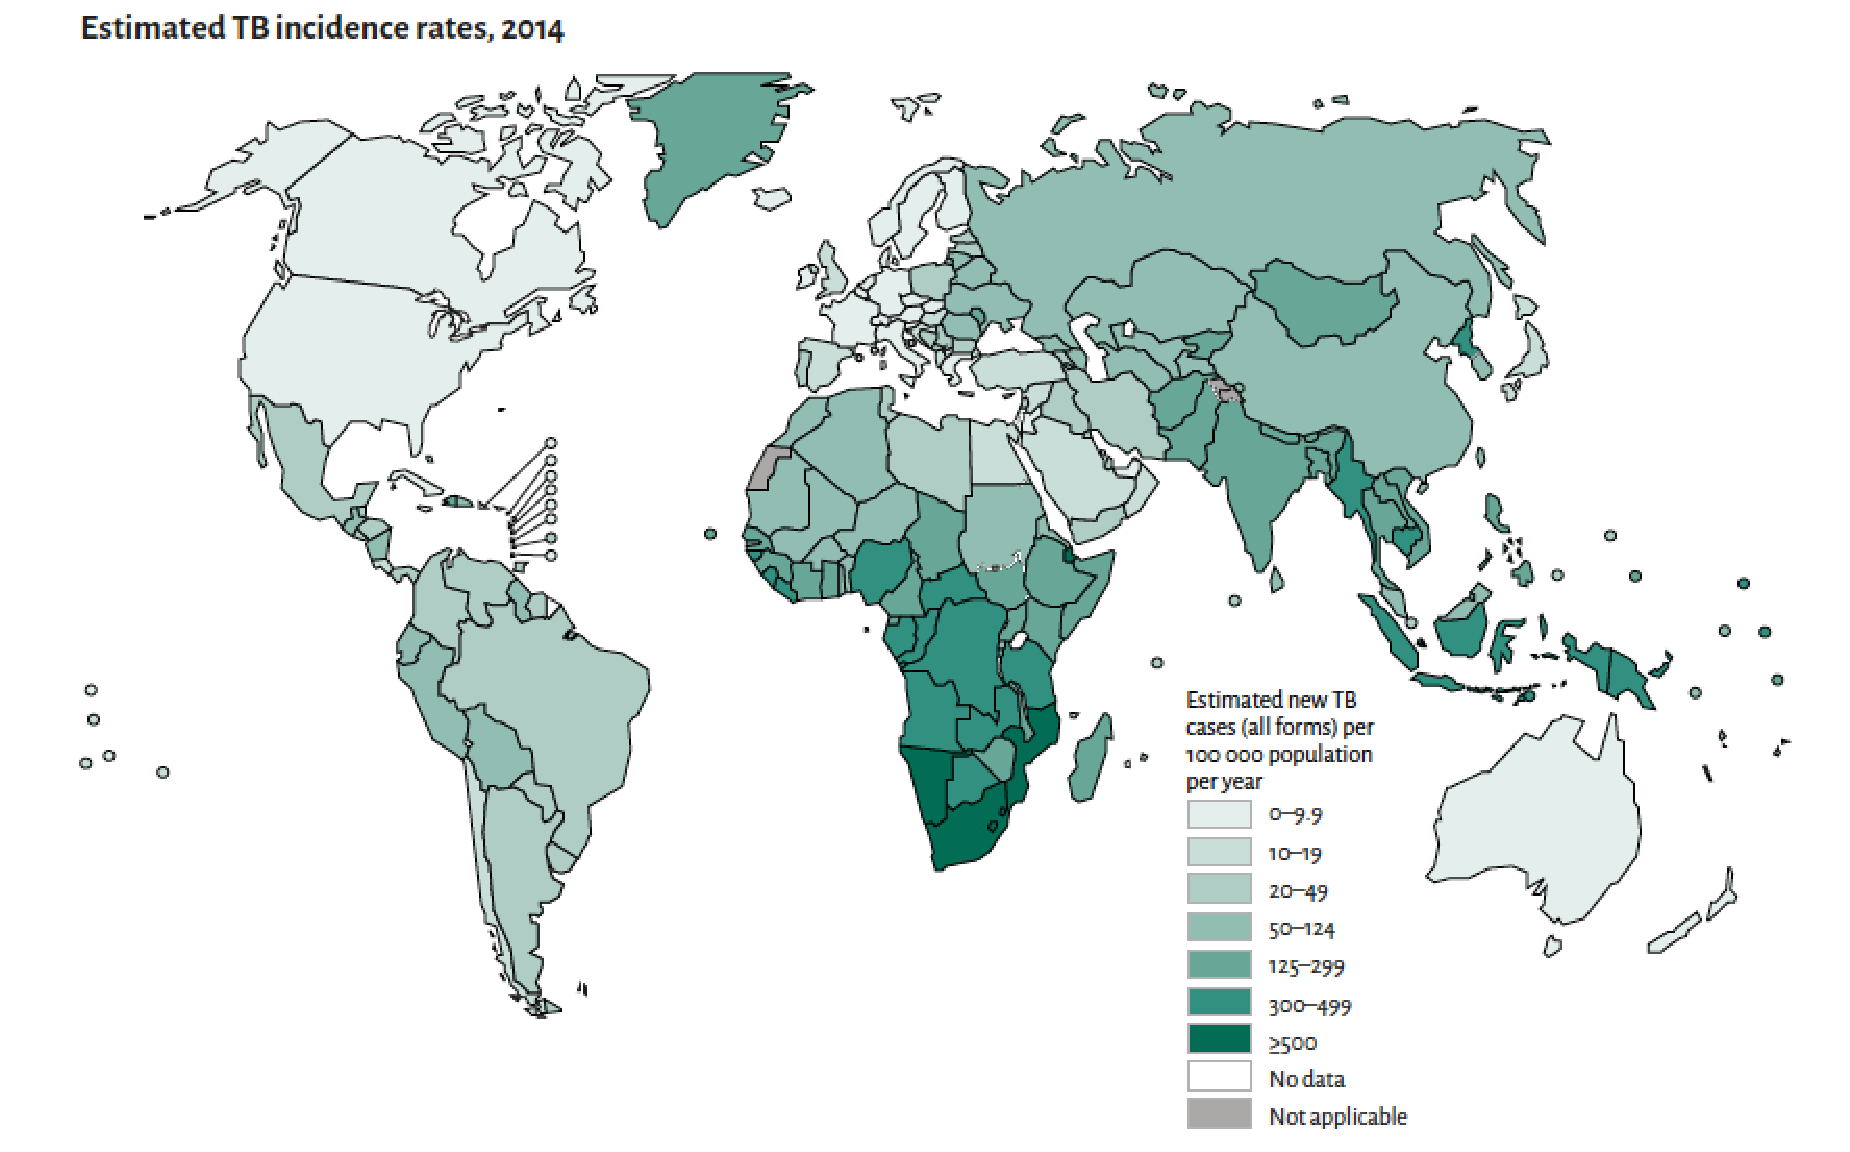
\includegraphics[width=0.9\linewidth]{../figures/map_incidence_tb.pdf}
	\caption[Estimated worldwide TB incidence rates in 2014]{Estimated worldwide TB incidence rates in 2014. Figure extracted from \cite{Lewandowski2015}.}
\label{fig:map_incidence_tb}
	
	\vspace*{4mm}
\end{figure}

\par These strategies are essentially created to bridge the financing gap in Tuberculosis R$\&$D. Next section focuses on specific methodologies and tools applied to perform research in this disease. Particular attention will be given to computer aided strategies applied to the TB research and discovery field. 

\subsubsection{Research strategies against MTB.}\label{mtb_research}

\par Beyond the funding problems of research against MTB, there are numerous technical challenges in identifying new antitubercular compounds \cite{Zuniga2015}. One the main difficulties is the extremely slow growth rate of \textit{Mycobacterium tuberculosis} as this is ultimately reflected in the rate of progress of discovery research. Another aspect is associated with the nature of the bacteria; MTB is a respiratory pathogen, and therefore has to be handled under strict safety conditions (Bio-safety Level 3) requiring expensive specialist facilities. Moreover, MTB have a very unusual cell wall that impedes many compounds from penetrating into the cell \cite{Brennan2003}. Additionally, this bacteria has efflux pumps that transport compounds out of the cell and that have been implicated in resistance to antibiotics \cite{Rodrigues2012}. To make things worse, anti-tubercular drugs need to be safe for periods over 6 months, or even longer periods when dealing with MDR-TB or XDR-TB, without significant side effects or drug-drug interactions. 
\par The search for new anti-tubercular compounds is therefore a extremely challenging task. Researchers are employing many different approaches in parallel including HTS and computational methods. HTS aims to find new molecular entities that may lead to the development of new antibacterial treatments. One of these HTS approaches is the \textit{cell based phenotypic screening}, which represents an efficient approach to identify anti-bacterial compounds and elucidate novel targets \cite{Manjunatha2015}. Some phenotypic screenings are also combined with toxicity assays to find those compounds with high anti-tubercular activity and positive PK profile \cite{Ballell2013}. Other HTS approaches aim at identifying highly potent molecules against an essential MTB target \cite{Park2015, Arora2014}.  Computational methods are essential in the analysis of the vast amount of data generated by HTS providing a tool to identity those candidate molecules amenable to be optimized in future stages. 

\subsubsection{In-silico approaches in TB}

\par Similarly to many other diseases, CADD methods play a substantial role in the Tuberculosis R$\&$D field. Uncountable \textit{in-silico} methods have been published over the last decade, each of them applying different strategies to solve a specific biomedical question. However, all of them pursue the very same goal: fueling drug discovery against TB. Table \ref{table:table_mtb_methods} contains some remarkable \textit{in-silico} resources for the fight
against TB. The purpose of these resources is very diverse. One popular resource is targetTB, which consist on an open-source pipeline to identify targets in MTB \cite{Raman2008a}. Similarly, \cref{mtb_results} presents how the combination of three orthogonal approaches can help to identify the molecular targets of novel anti-tubercular compounds. Other resources, such as TDRtargets \cite{Crowther2010} (\url{http://tdrtargets.org/}) and CCD-TB \cite{Ekins2010},  blend a target detection tool with a publicly accessible database of known existing targets and anti-microbial compounds. Some methods, on the other hand, are focused on providing insights into a specific problem in TB treatment. Such is the case of the computational detection of Comtan as a potential agent in the treatment of MDR-TB and XDR-TB \cite{Kinnings2009}, or the examples from \cite{DeJonge2007} and \cite{Kumar2009}. Most of these resources take advantage of Tuberculist \cite{Lew2011}, a database of experimentally measured gene essentiality in MTB; and TuberQ \cite{Radusky2014}, which contains information about MTB protein druggability. Is such the importance of computational resources in TB research that recently a Mobile app, called TB-Mobile \cite{Ekins2013, Clark2014}, was published. TB-Mobile provides an agile way to interact with TB data and it includes some chemoinformatics tools for clustering and finding new molecular targets to known anti-tubercular compounds. This app is therefore pushing the boundaries of science on mobile devices in several important ways, and could set up a milestone in bringing mobile apps into the computational biology research field.

\par Overall, \textit{in-silico} methods play an important role in the research against tropical infectious diseases. Particularly, TB benefited enormously from the contribution of such methods and therefore they are partly responsible of the improvement in the prognosis of the disease. 



\tabulinesep=1.4mm{
\begin{longtabu} to \textwidth {|| X | X |  p{4cm} | X ||}
 

 
 %\begin{adjustbox}{width=1\textwidth, totalheight=\textheight,keepaspectratio}
 %\small
 %\begin{tabularx}
 \hline
 \tr\textbf{Type of method}\br &\tr\textbf{Name}\br  & \tr\textbf{Resource description}\br & \tr\textbf{Reference(s)}\br\\  
\hline
 Target identification pipeline & TargetTB & Target prioritization in TB thorough a computational pipeline   & \cite{Raman2008}  \\ 
 \hline
 Database &  TDRtargets & Database and method for identification of potential MTB targets & \cite{Crowther2010} \\
 \hline   
 Application of bioinformatics tools & -  & Drug repositioning applied to MDR-TB and XDR-TB & \cite{Kinnings2009}  \\
 \hline
  Database &  CDD-TB & Database of anti-tubercular compounds reported from HTS alongside computational models to analyze the data  &   \cite{Ekins2010}  \\
 \hline
 Application of bioinformatics and chemoinformatics tools & -  & Identification of the MTB targets of bio-active anti-tubercular compounds using three orthogonal \textit{in-silico } approaches & \cite{Martinez-Jimenez2013, Rebollo-Lopez2015}   \\ 
 \hline
  Application of bioinformatics tools &  -  & Homology modelling and virtual doking applied to ligand-protein interaction prediction & \cite{DeJonge2007} \\
 \hline
 Application of chemoinfomatics tools & TB Mobile &   Mobile app that provides a platform to interact with data collected from CDD-TB & \cite{Ekins2013, Clark2014} \\
 \hline 

     Application of bioinformatics and chemoinformatics tools & - & Identification of Enoyl acyl carrier protein reductase binders using a 3D-QSAR approach & \cite{Kumar2009} \\
   \hline
    Application of bioinformatics tools & - &  Interactome computational analysis to identify potential mechanisms of drug resistance to TB therapies & \cite{Raman2008} \\
   \hline
    Database & Tuberculist &  Database of experimentally measured gene essentiality & \cite{Lew2011} \\
   \hline
    Database & TuberQ &  MTB protein druggability database  &  \cite{Radusky2014} \\
   \hline
   \caption[Table containing multiple computational resources used in the discovery and research against TB]{Table containing multiple computational resources used in the discovery and research against TB} 
   \label{table:table_mtb_methods} 
%\end{tabularx}



\end{longtabu}}



\subsection{Drug discovery in cancer}\label{dd_cancer}

\par Over the previous sections, we discussed how tuberculosis, among other infectious diseases, has significantly benefited from the application of \textit{in-silico} methods. The importance of computational methods is also observed in other diseases research and discovery programs. Interestingly, bioinformatics-assisted diseases include cancer. Cancer research has significantly improved due to development of large-scale genomics techniques alongside computational methods to deal with the massive amount of generated data. The next section discusses about advances in cancer treatment, focusing on targeted cancer therapy, a particular type of cancer treatment. The emergence of targeted cancer therapies significantly changed the reality of cancer treatment. Unlike classic chemotherapy agents, targeted therapies perform their activity by specifically attacking proteins involved in the growth, progression, and spread of cancer. However, clinical benefits associated to targeted therapies are often temporal due to the emergence of drug resistance. Next sections will also discuss about this problem, explaining the molecular mechanisms leading to the emergence of drug resistance. Finally, \cref{blending} presents a computational model aiming to assist in the choice of non-resistant targeted cancer therapies. 

\subsection{Targeted cancer therapy}\label{targeted therapies}


\par Cancer is one the leading causes of morbidity and mortality worldwide. In 2012 there were more than 14 million new cases and 8.2 million cancer related deaths. Moreover, the cancer global burden is expected to rise by about 70$\%$ over the next 20 years \cite{WHO_CANCER}. Intravenous cytotoxic chemotherapy has traditionally prevailed as the main therapeutic choice in cancer treatment. Chemotherapy drugs target rapidly dividing cells, including cancer cells and certain normal tissues.  Hence, the lack of specificity of the chemotherapy treatment leads to strong side side effects such as hair loss, gastrointestinal symptoms, fatigue or myelosuppression, among others.  In the past decade, however, the arrival of targeted cancer therapies have dramatically transformed cancer treatment. Targeted cancer therapies are drugs designed to specifically interfere with molecules necessary for tumorigenesis. The higher specificity associated to these drugs makes them a more efficient and less harming alternative for cancer treatment. Although chemotherapy remains the treatment of choice for many malignancies, targeted therapies are now a essential component of treatment for many types of cancer, including breast, colorectal, non-small cell lung cancer (NSCLC), as well as lymphoma, several classes of leukemia, and multiple myeloma. There are two main types of targeted cancer therapies, monoclonal antibodies and small molecule inhibitors.

\subsubsection{Monoclonal antibodies}

\par  Monoclonal antibody-based therapy for cancer has become established over the past 15 years. Monoclonal antibodies are target specific, which means that they exclusively target only one protein. Moreover, their protein target has to be extra cellular, as the antibodies cannot enter the cell through the plasma membrane. Monoclonal antibodies can kill tumour cells throughout multiple mechanism of action \cite{Scott2012}. One of the classic mechanism consist on direct action of the antibody on the target protein. An example of this class is the monoclonal antibody cetuximab, an epidermal growth factor receptor (EGFR) inhibitor used in EGFR-positive colorectal cancer \cite{Jonker2007} and squamous cell carcinoma of the head and neck (SCCHN) \cite{Tejani2010}. Another mechanism consist on the activation of the immune system response to kill cancer cells. Immunotherapies are becoming increasingly popular and its currently one of the most promising fields of cancer research.  Examples of this class include the immune checkpoint inhibitors  pembrolizumab (PD-1), atezolizumab (PDL-1) and ipilimumab (CTLA-4) \cite{Postow2015}; or the CD52 antibody alemtuzumab \cite{Demko2008}. Tumor vascularization and stroma have also been targeted by antibody-based therapies. For example, bevacizumab is a monoclonal antibody that blocks angiogenesis by targeting the vascular endothelial growth factor receptor (VEGFR) \cite{Ferrara2004}. It is currently used as a single agent or in combination with chemotherapy to treat certain types of advanced cancer, including colorectal, NSCLC, glioblastoma or kidney cancer \cite{Keating2014}. Finally, several conjugated antibodies have been approved to treat cancer. An example of this class is ibritumomab tiuxetan, a yttrium-90-conjugated monoclonal antibody to CD20, for patients with relapsed B-cell non-Hodgkin's lymphomas. This drug combines the monoclonal antibody ibritumomab in conjunction with the chelator tiuxetan, to which radioactive isotope is added \cite{Witzig2002}. Undoubtedly, antibody-based cancer therapies have significantly contributed to the improvement of cancer survival. However, these therapies have still important limitations which prevents them for broader application. One of the major limitations is the temporally efficacy of some treatments. Patients with malignant tumors may not achieve a long-term therapeutic effect consequence of the multiple tumour escape mechanisms \cite{Scott2012}. Deeper understanding of the tumor biology may provide insight into selection of patients who are suited to a specific antibody treatment. In summary, monoclonal antibodies have shown a great potential in the treatment of cancer. However, there are important limitations that need to be addressed to increase the clinical impact of this type of treatment.  

\subsubsection{Small molecule kinase inhibitors}\label{kinases}

\par Small molecule inhibitors is the second main class of targeted cancer therapy.  Unlike monoclonal antibodies, they can penetrate into the cell through the plasma membrane. Small molecule targeted cancer therapies mainly focus on inhibiting protein kinases. In fact, kinases have been established as promising drug targets for the treatment of various types of human disease because of their essential roles in signal transductions and regulation of a range of cellular activities. However, the vast majority of these targets are being investigated for the treatment of cancer \cite{Zhang2009}.  Over the last years,  many kinases have been found to be deeply involved in the processes leading to tumorigenesis. Depending of their role in cancer progression we can classify small molecule kinase targets into different groups.  First, there are kinases that have become insensitive to normal regulatory mechanisms. The altered activity of such kinases can be the consequence of genetic alterations (e.g., mutations or translocations) or epigenetic changes (e.g., gene amplification, increased expression) and are considered to be oncogenic. The constitutive activity of this class of kinase target makes them essential for survival and/or proliferation of the cancer cell. This phenomenon is known as oncogene addiction \cite{Weinstein2006}, and makes the cancer cell exceptionally susceptible to the oncogene kinase inhibitor. One of best examples of this phenomenon is the activating V600E BRAF mutation. About 50$\%$ of melanomas harbour this oncogenic mutation \cite{Ascierto2012}. Currently, there are two small molecules FDA approved inhibitors that specifically target the BRAF V600E-mutated metastatic melanoma, vemurafenib \cite{Bollag2010} and dabrafenib \cite{Gibney2013}. Inhibiting mutationally activated kinases (i.e., oncogenic kinases) has resulted in the most dramatic clinical responses \cite{Zhang2009}.  A second class of target kinases is composed by those non-oncogenic kinases whose presence is preferentially required for the survival and/or proliferation of tumor cells.  These kinases are usually located in key signalling pathways downstream of cancer oncogenes. Examples of this type of targets include MEK1 and MEK2 (also known as MAP2K1 and MAP2K2), which are targeted by several small molecule inhibitors such as trametinib or cobimetinib. Combinations of these inhibitors with oncogene inhibitors led into a significant improvement in patient survival compared with single treatment regime in melanoma \cite{Flaherty2012, Flaherty2012a}. Another class of kinase targets are those highly expressed in the tumor stroma and that are required for different stages of tumor formation and development in the human host. Examples of this class include the inhibition of VEGFR by pazopanib or by other small molecule inhibitors \cite{Ivy2009}.
 
 \par Protein kinases are defined by their ability to catalyse the transfer of the terminal phosphate of ATP to a substrate that usually contains a serine, threonine or tyrosine. They share a highly conserved arrangement of secondary structure elements that fold into a bi-lobed catalytic core structure (N-terminal lobe and C-terminal lobe), with ATP binding site located in a deep cleft located between the two lobes \cite{Manning2002} (Figure \ref{fig:kinase_general_conformation}). The ATP adenine ring forms hydrogen bonds with the kinase hinge region (\textit{i.e.}, the segment that connects the amino and carboxy terminal kinase domains), while the ribose and triphosphate groups of ATP bind in a hydrophilic channel adjacent to the ATP binding site that contains conserved residues essential to catalysis. Additionally, kinases have a conserved activation loop, which regulates the kinase activity and that contains a extremely conserved DFG motif (\textit{i.e.}, aspartic acid, phenylalanine and glycine) at the start of the loop. The structural disposition of the activation loop switches between the active and inactive conformations of the protein kinase \cite{Manning2002}. Since the catalytic mechanism requires the exact positioning of highly conserved active site residues, the kinase active state is rigid and highly conserved. In contrast, kinase inactive states are structurally highly diverse and dynamic \cite{Muller2015}. Furthermore, the kinase ATP binding site contains a highly flexible phosphate-binding loop (P-loop). In many kinases the P-loop contains an aromatic residue that points upward in the active kinase state, enabling the binding of ATP. Finally, kinases contain a key residue in the ATP-binding site known as \textit{gatekeeper}. This residue is located close to the hinge region and controls the access of small molecule inhibitors to a hydrophobic pocket in the active site that is not contacted by ATP \cite{Lui1998} (Figure \ref{fig:kinase_general_conformation}).  
 
 \begin{figure}[htbp]
  
  \centering
    
   
	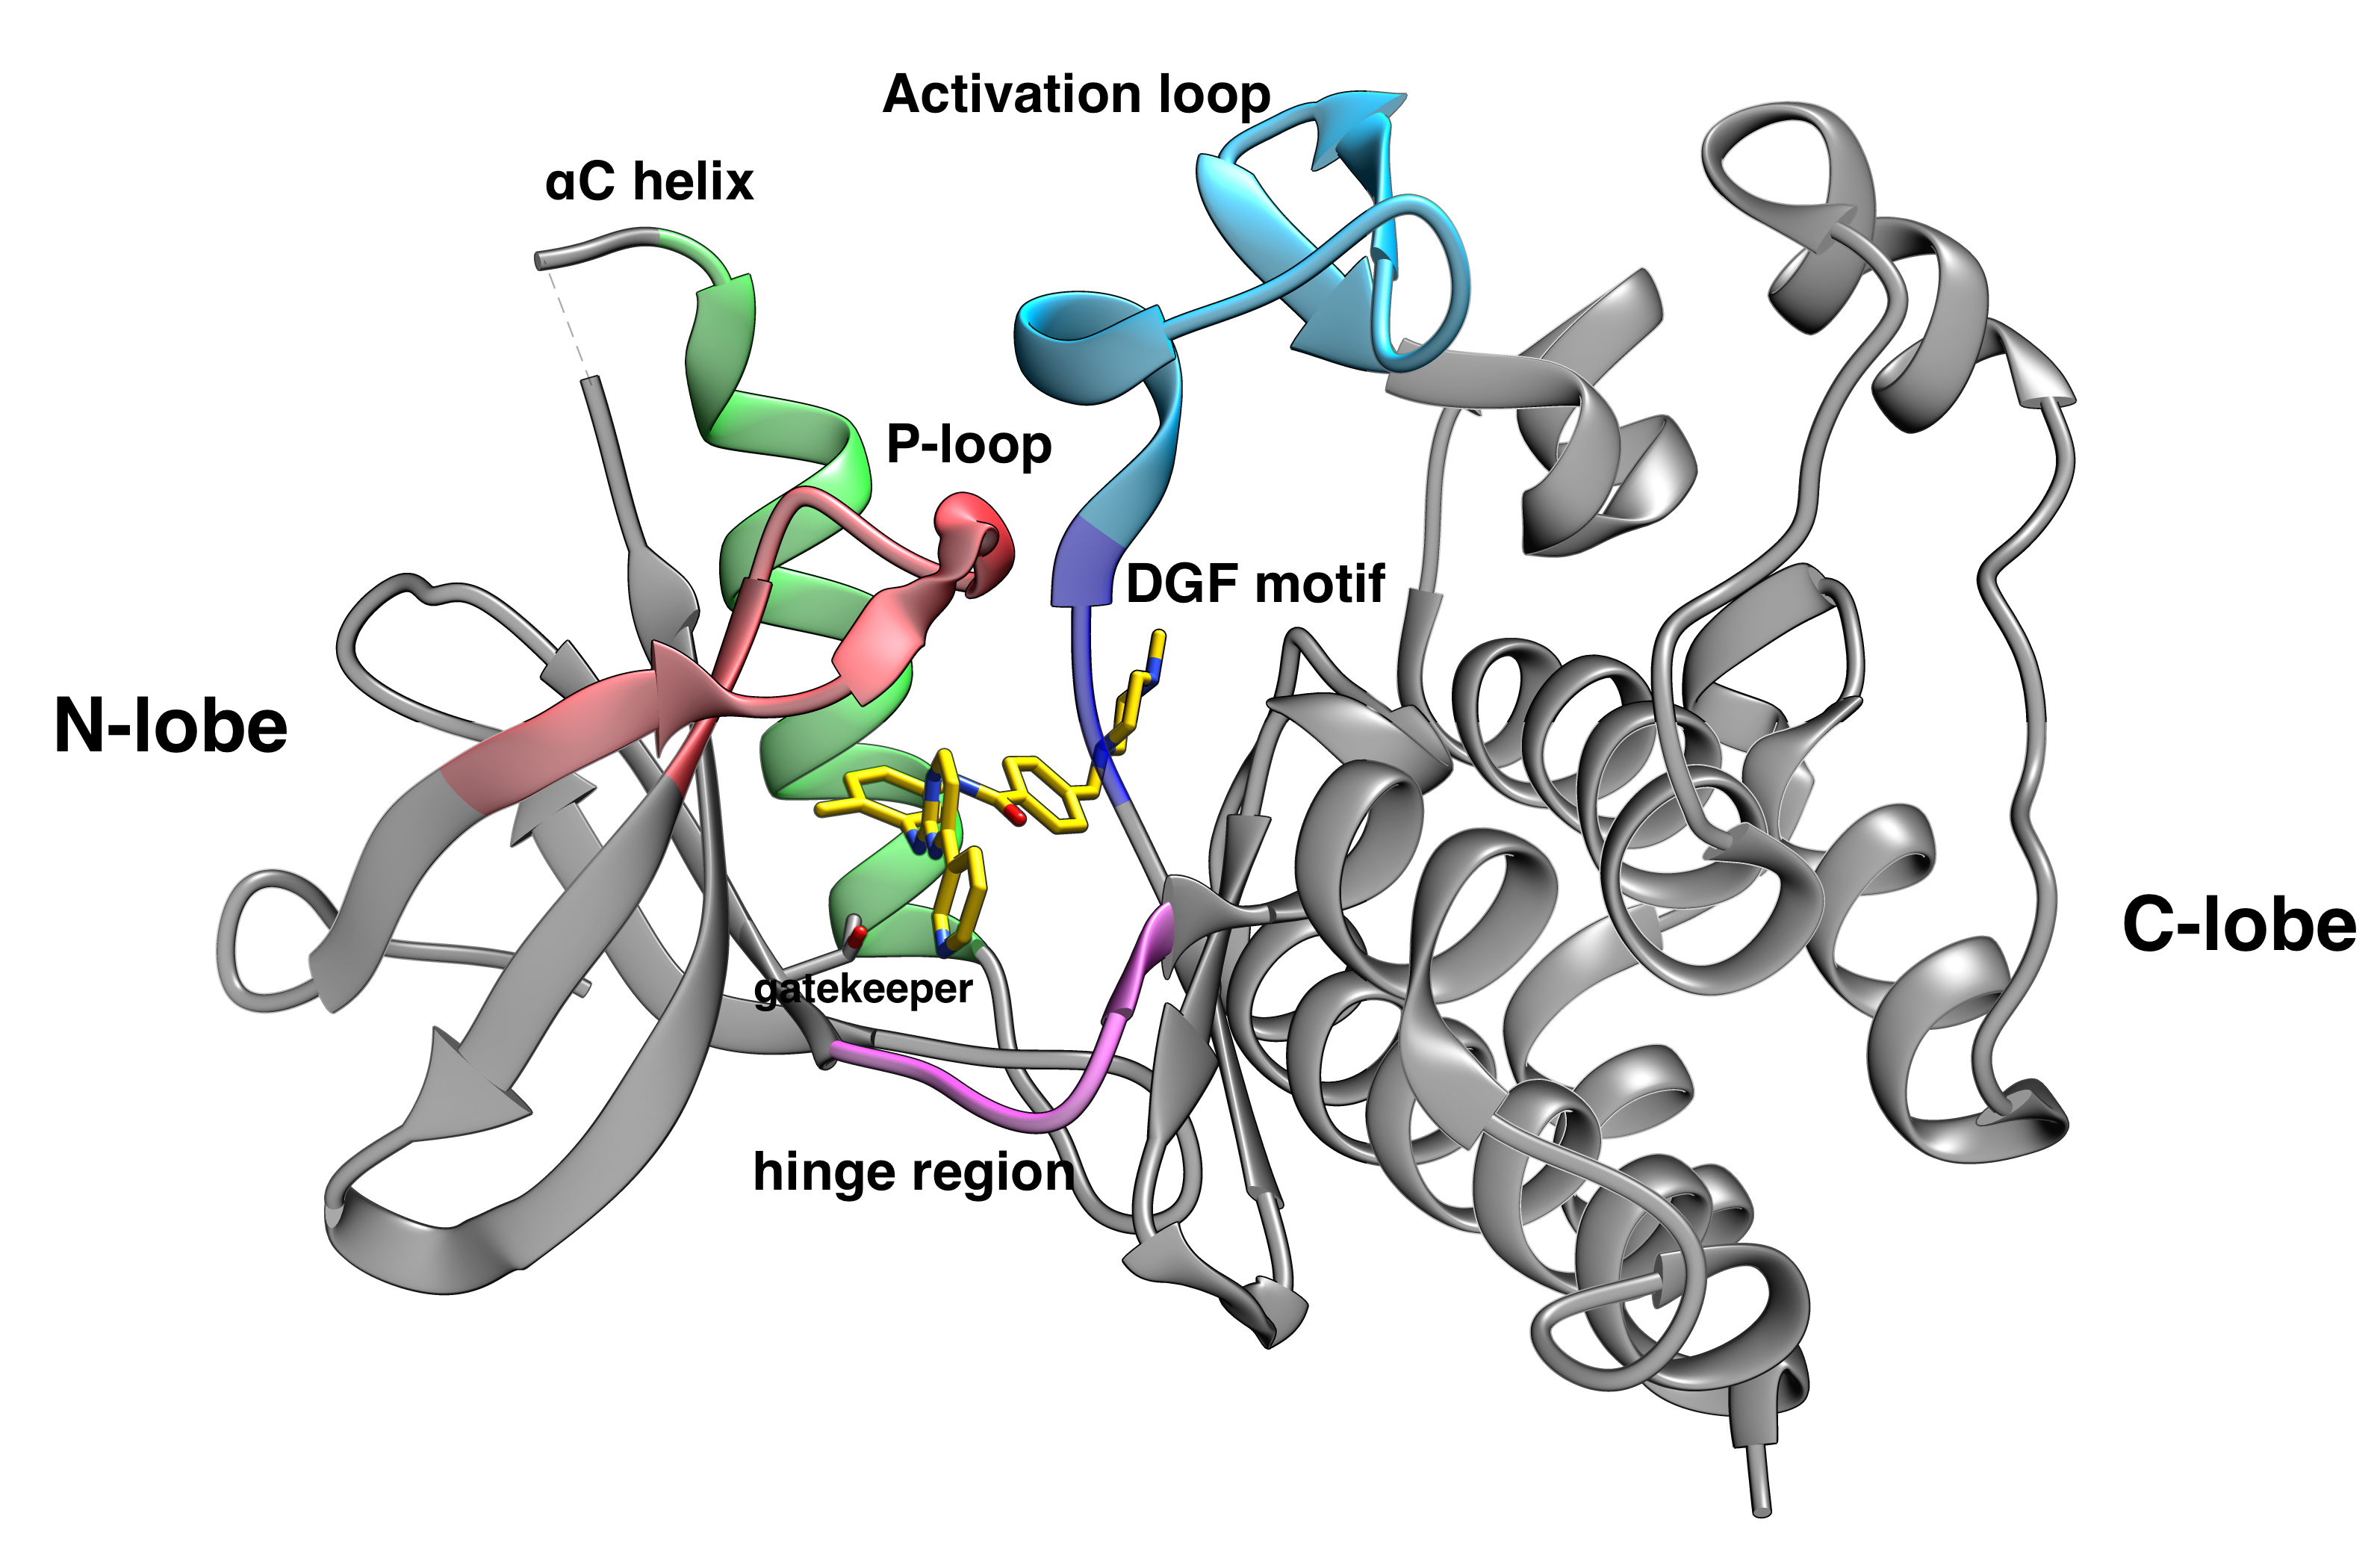
\includegraphics[width=1\linewidth]{../figures/kinase_structure.png}
	\caption[Schematic representation of the different structural regions of protein kinases]{3D structure of ABL1 kinase in complex with imatinib displaying the different structural regions of protein kinases. The structure represents the typical kinase inactive DGF-out conformation. The protein is represented as ribbons and the ligand as sticks. The activation loop is coloured in cyan, the DGF motif in blue, the P-loop is coloured in red, the hinge region in purple and the $\alpha$C helix in green. PDB accession code 2HYY.}
	\label{fig:kinase_general_conformation}
	
\end{figure}
\par Most of the current small molecule kinase inhibitors are ATP-competitive that mimic the ATP binding mode. However, depending of their specific binding mode small molecule protein kinase inhibitors can be classified into multiple classes:

 \begin{enumerate}
 
\item \textbf{Type I inhibitors}. This type of ATP-competitive inhibitor binds the active conformation of the protein kinase. As mentioned above, the kinase active state is well defined and it is more rigid than inactive kinase states. Moreover, is very conserved among kinases making the development of selective type I inhibitors a very challenging task. The specificity is therefore given by unusual active site features such as rare amino acids in conserved positions, inserts/deletions, and, in some cases, residues that can be targeted by irreversible inhibitors. Additionally,  small gatekeeper residues, such as threonine, can provide access to a hydrophobic \textit{back pocket} not contacted by ATP \cite{Noble2004}. Type I inhibitors typically consist of a heterocyclic core scaffold that occupies the adenine binding site alongside side chains that occupy the adjacent hydrophobic regions (Figure \ref{fig:type_inhibitors}). Examples of this class include the EGFR inhibitors gefitinib and erlotinib, the BRAF V600E-mutant inhibitor vemurafenib, the anaplastic lymphoma kinase (ALK) inhibitor crizotinib or the Bcr-Abl tyrosine kinase inhibitor dasatinib. The complete list of type I inhibitors is shown in Table \ref{table:table_inhibitors}. 

\item \textbf{Type II inhibitors}. Type 2 kinase inhibitors recognize the inactive conformation of the kinase. The most frequent conformation recognized by type 2 inhibitors is the so-called DFG-out. This conformation is created by a rearrangement of the activation loop that creates an extended and flexible binding pocket adjacent to the ATP binding site (Figure \ref{fig:type_inhibitors}). The high degree of flexibility generated by this conformation suggests that inhibitors targeting such states should have a better chance of being selective. However, recent comprehensive analysis of type II selectivity revealed that many kinases can assume this inactive state and that type II inhibitors may not be intrinsically more selective than type I inhibitors \cite{Inhibitor2016}. The original discovery that inhibitors such as imatinib and sorafenib bind in the type 2 conformation was serendipitous, but subsequent analysis of multiple type 2 kinase inhibitor revealed that most of them share a similar binding pattern \cite{Inhibitor2016}. Other examples of type II kinase inhibitors include the BCR-ABL kinase inhibitors nilotinib or ponatinib. The complete list of FDA approved type II inhibitors is shown in Table \ref{table:table_inhibitors}. 

\item \textbf{Targeting P-loop conformations}. In kinase-inhibitor complexes, the P-loop may fold into the ATP-binding site, forming aromatic stacking interactions with the inhibitor \cite{Guimaraes2011}. An additional characteristic of folded P-loop conformations is the induction of a large binding cavity between the P-loop and the $\alpha$C helix (Figure \ref{fig:type_inhibitors}). This binding cavity is present in many structures with folded P-loops and has been explored, for the first time, by the selective ERK1/2 inhibitor SCH772984 \cite{Morris2013}. Multiple kinases can adopt a folded P-loop conformation, which unique geometric features of this binding mode may lead into the development of selective inhibitors for these kinases. Nevertheless, none of FDA approved drugs adopt this conformation, and therefore a broader general demonstration of this inhibitor binding mode is still necessary. 
\begin{figure}[htbp]
	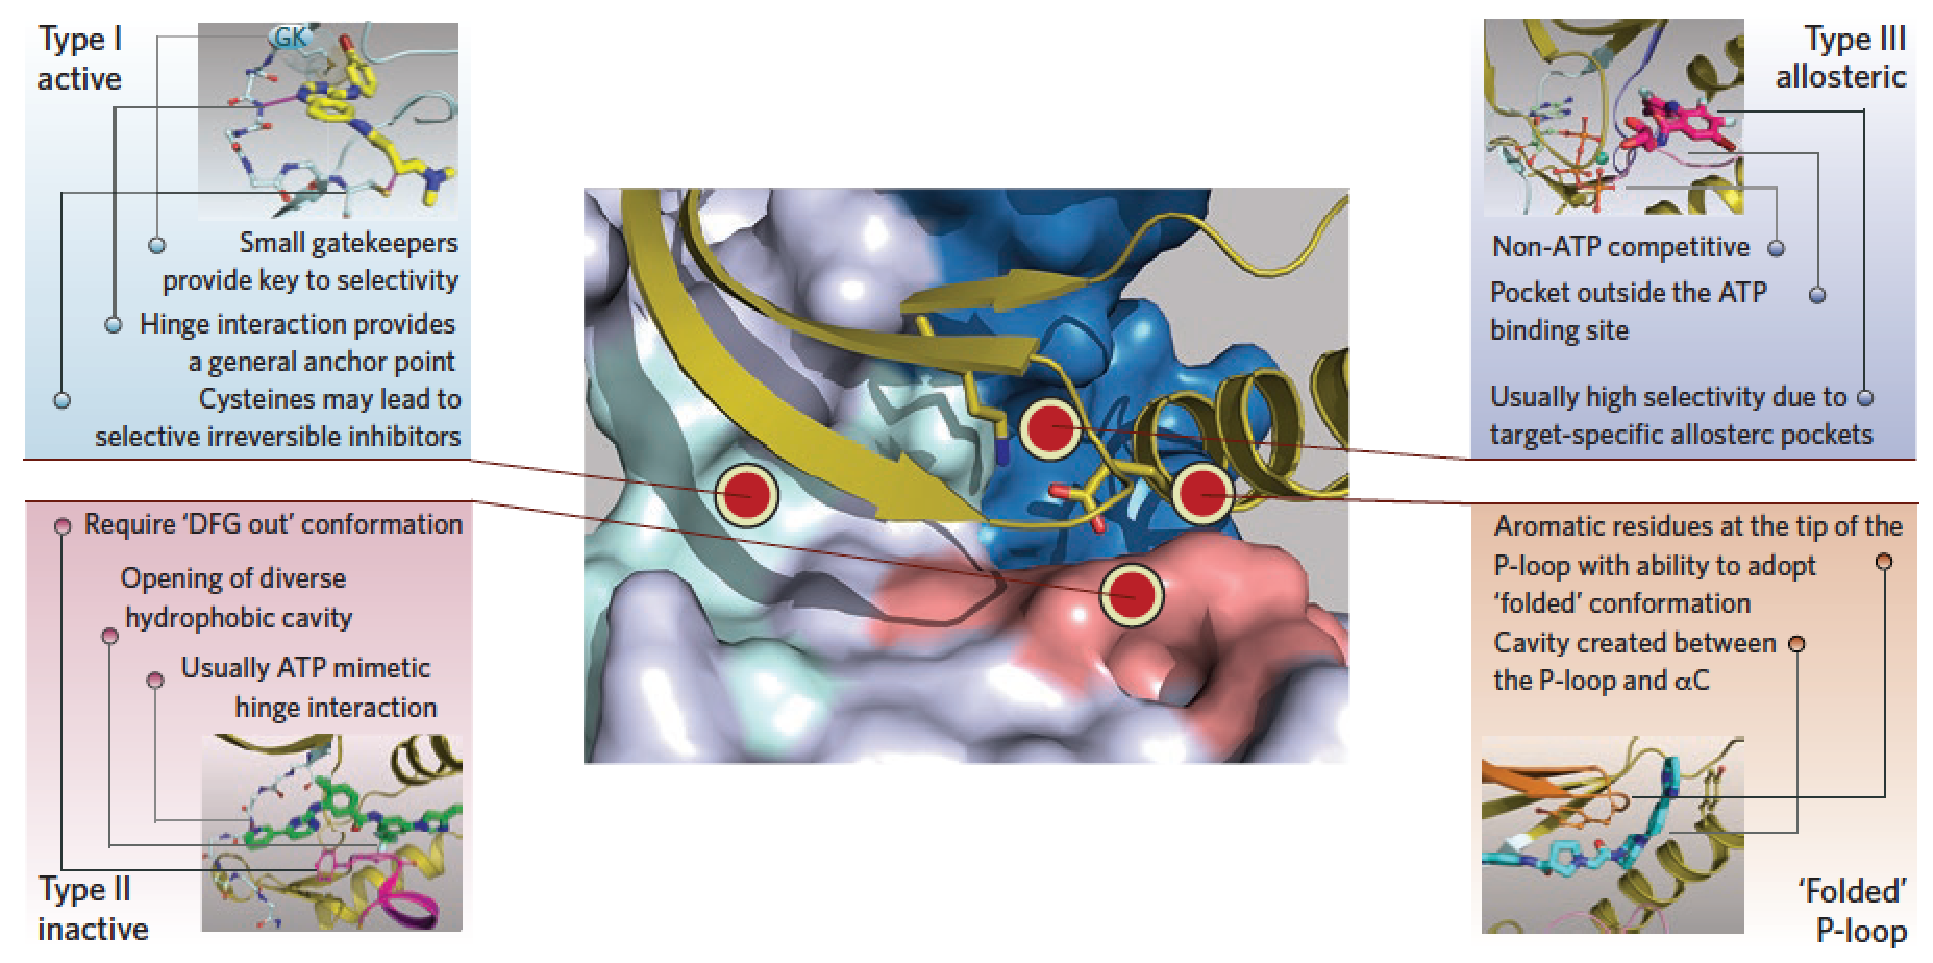
\includegraphics[width=1\linewidth]{../figures/type_kinases_inhibitors.pdf}
	\caption[Structural features of the canonical classes of small molecule kinase inhibitors]{Structural features of the canonical classes of small molecule kinase inhibitors. The center panel shows the main interaction sites of different inhibitors types. The side panels show the specific structural features of each of the binding modes. Figure extracted from \cite{Muller2015}.}
	\label{fig:type_inhibitors}
	\vspace*{4mm}
\end{figure}
\item \textbf{Type III allosteric inhibitors}. Type III kinase inhibitors are non ATP-competitive inhibitors binding the kinase in a allosteric site (\textit{i.e.}, a site distinct from the enzyme active site that can bind a ligand) and modulating kinase activity in an allosteric manner. Allosteric inhibitors tend to exhibit the highest degree of selectivity since they exploit binding sites and regulatory mechanisms that are unique to each particular kinase (Figure \ref{fig:type_inhibitors}). Most allosteric kinase inhibitors have been discovered serendipitously, and currently there is no general strategy for identifying such compounds. The best examples of this class are the MEK1/MEK2 allosteric inhibitors trametinib and cobimetinib, which occupy a pocket adjacent to the ATP binding site. 

\item \textbf{Covalent inhibitors}. The last class of kinase inhibitors are those capable of forming an irreversible, covalent bond to the kinase active site, most frequently thorough the reaction with a nucleophilic cysteine residue \cite{Cohen2005}. Most of the covalent kinase inhibitors have been developed by structure-guided incorporation of an electrophilic group into an inhibitor that already had sub-micromolar binding affinity \cite{Potashman2009}. Although a large number of kinases have cysteine residues in and around the ATP-binding site, there are not conserved cysteines residues across the human kinome \cite{Liu2013a}. This lack of conservation has been used to develop selective irreversible inhibitors of kinases habouring cysteine residues in the ATP-binding site. However, cross-reactivity of cysteine-reactive groups can lead to non-selective reactions with off-target proteins, which eventually gives rise to increased toxicity and lack of target specificity \cite{Barf2012, Liebler2008}. Examples of FDA approved irreversible inhibitors include the Bruton's tyrosine kinase inhibitor (BTK) Ibrutinib or the EGFR inhibitor afatinib.
 
 
\end{enumerate}  
 
 
 
 
 

   

\renewcommand{\arraystretch}{1.2}
\begin{adjustbox}{max width=\textwidth}
\begin{threeparttable}[htbp]

 \centering

 %\begin{tabular}{*{4}{|| p{2cm} | p{4cm}  |  p{3cm} | p{1cm} } ||} 
 \begin{tabular}{*{4}{|| c | c  |  c | c  ||}} 
 \hline
 \tr\textbf{Compound name}\br &\tr\textbf{Pharmacological Target}\br  & \tr\textbf{Binding mode}\br & \tr\textbf{First FDA approval}\br\\  

\hline
 Imatinib & ABL1 &  Type II   & 2001  \\  
\hline
 Gefitinib & EGFR &  Type I   & 2003  \\  
 \hline
 Erlotinib & EGFR &  Type I   & 2005  \\  
 \hline
 Sorafenib & VEGFR, PDGFR, BRAF, etc. & Type II & 2005  \\  
 \hline
 Dasatinib & ABL1 &  Type I   & 2006  \\ 
 \hline
 Sunitinib & VEGFR &  Type I   & 2006  \\
 \hline
 Nilotinib & ABL1 &  Type II   & 2007  \\ 
 \hline
 Lapatinib & EGFR, HER2 &  Type I and II   & 2007  \\  
  \hline
 Pazopanib & VEGFR, PDGFR, c-KIT, etc.&  Type I and II   & 2009  \\ 
 \hline
 Crizotinib & ALK, ROS1 &  Type I   & 2011  \\ 
 \hline
 Vemurafenib & BRAF &  Type I   & 2011  \\ 
 \hline
 Ruxolitinib & JAK1/2 &  Type I   & 2011  \\  
 \hline
 Vandetanib & VEGFR &  Type I   & 2011  \\ 
  \hline
 Bosutinib & BCR-ABL1 &  Type I   & 2012  \\ 
  \hline
 Tofacitinib & JAK3 &  Type I   & 2012  \\
  \hline
 Axitinib & VEGFR, PDGFR, c-KIT &  Type I   & 2012  \\ 
  \hline
 Cabozantinib & c-MET &  Type II   & 2012  \\  
  \hline
 Regorafenib & VEGFR, PDGFR, etc. &  Type II   & 2012  \\  
  \hline
 Ponatinib & ABL1 &  Type II   & 2012  \\   
  \hline
 Dabrafenib & BRAF &  Type I   & 2013  \\     
 \hline
 Trametinib & MEK1/2 &  Type III   & 2013  \\ 
  \hline
 Afatinib & EGFR &  Type I, Irreversible  & 2013  \\ 
  \hline
 Ibrutinib & BTK &  Type I, Irreversible  & 2013  \\
  \hline
 Idelalisib & PI3K-delta &  Type I   & 2014  \\
  \hline
 Nintedanib & VEGFR, PDGFR, etc.&  Type II   & 2014  \\
 \hline 
 Ceritinib  &   ALK, MET &  Type II  & 2014 \\
 \hline 
 Lenvatinib  &   VEGFR, PDGFR, c-KIT, FGFR, etc. &  Type V \tnote{\textdagger}  & 2015 \\
 \hline 
 Palbociclib  &   CDK4/6 &  Type I  & 2015 \\
 \hline
 
 \end{tabular} 
 
  \begin{tablenotes}
  
  \footnotesize
\item[\textdagger] In a recent publication, lenvatinib was proposed as a special class of kinase inhibitors (the so-called type V inhibitors). Compounds of this class are those binding both the ATP-binding site and the neighboring allosteric region in kinases with DFG-in conformation \cite{Okamoto2015}. 
\end{tablenotes}



\caption{FDA approved kinase inhibitors alonsgide their pharmacological target, binding mode and year of FDA approval.}
\label{table:table_inhibitors} 

 \end{threeparttable}
\end{adjustbox} 
 
\par The approval of imatinib in 2001 radically transformed the treatment of Philadelphia chromosome-positive (Ph+) chronic myelogenous leukemia (CML). Since then, more than 27 different small molecule kinase inhibitors have been approved by the FDA (Table \ref{table:table_inhibitors}), and many others are currently in clinical trials for the treatment of cancer. Despite of their great success in cancer treatment, small molecule kinase inhibitors suffer from major limitations that need to be addressed to improve their clinical impact. Next, I outline some of their most important challenges and limitations:  

\begin{enumerate}

\item Of the total 538 estimated human kinases \cite{Manning2002}, only a few, and most of them belonging to the tyrosine kinase group, have been pharmacologically targeted by small molecule inhibitors. It is thus necessary to increase the spectrum of clinically targeted kinases. Moreover, the increment of the number of targeted kinases would create new therapeutic opportunities for disorders where kinases play an important, but yet clinically unexplored role. 
\item Other important limitation is the lack of specificity of many small molecule kinase inhibitors. This is mainly consequence of the high structural conservation of the ATP-binding site in kinases, which causes that a large number of inhibitors interact with more than one target \cite{Davis2011}. The multitarget nature of many kinase inhibitors gives rise to severe side effects that dramatically restricts its applicability in the clinics. Fostering the development of type III allosteric inhibitors would lead into more selective inhibitors preventing the appearance of unexpected toxicities.  
\item Related to the previous point, the mechanistic basis of unexpected toxicities observed during the preclinical and clinical stages need to be studied more rigorously. Improved documentation of kinase inhibitor specificity and observed toxicities would provide a valuable database for understanding whether there are particular kinases of which inhibition should be particularly avoided \cite{Zhang2009a}.
\item The most important limitation of small-molecule kinase inhibitors, in particular, and targeted cancer therapies, in general, is the rapid acquisition of drug resistance. The duration of clinical benefits is frequently short, which dramatically restricts the utility of many targeted cancer therapies. The next section will focus on the mechanistic basis of resistance to targeted cancer therapies, with particular emphasis on mutations of kinase targets altering the efficacy of the treatment.    
 \end{enumerate}
 


\subsubsection{Resistance to targeted cancer therapies}\label{resistance}

\par Drug resistance is one of the major problems in cancer treatment. Resistance to both chemotherapy agents and targeted cancer therapies is hampering the success of many anticancer treatments. The advent of new high throughput genomic technologies and its combination with bioinformatics and systems biology approaches, have enhanced the understanding of the molecular events underlying treatment failure. However, we are still far from overcoming the emergence of drug resistance in cancer targeted therapies. One of the reasons leading to the complex drug resistance problem is the considerable amount of molecular mechanisms leading to drug resistance \cite{Holohan2013}. Some mechanisms of resistance for specific molecular targets share many features with the classic cytotoxic chemotherapy, while others, are genuine to the targeted cancer therapies. One of the classic mechanisms of resistance is caused by the pharmacokinetics properties (ADME) of the drugs, which added to the limited amount of drug that can be systemically administered confine the amount of drug reaching the tumor. That means that the concentration of drug that eventually reaches the cancer cells is lower than the one required to perform the desired antiproliferative activity \cite{Gottesman2002}. At the level of the tumor, various resistance mechanisms can operate, including activation of survival signalling pathways and the inactivation of downstream death signalling pathways \cite{Lowe2004}, oncogenic bypass and pathway redundancy \cite{Logue2012}, factors associated to the tumor microenviroment \cite{McMillin2013} or epigenetic alterations \cite{Maier2005}.
\par Importantly, alterations in the drug target is one of the most frequent mechanism of resistance in targeted cancer therapies. Increased expression of the molecular target reduces the effectiveness of inhibitors of these targets because more target molecules must be inhibited to have a effective therapeutic effect. For instance, the androgen receptor (AR) is genomically amplified in aproximately 30$\%$ of prostate cancers with acquired resistance to standard androgen deprivation therapy. In such cases, treatment using testosterone lowering drugs such as leuprolide and AR antagonists such as bicalutamide, is not effective and alternative treatments are thus necessary \cite{Koivisto1997}. 

\par Most of the small molecule targeted cancer therapies target oncogenic kinases that are responsible of the tumor proliferation and/or development (\cref{kinases}). Mutations of these oncogenic kinases can alter the binding of the small molecule kinase inhibitor giving rise to a reestablishment of the tumor proliferation activity. Moreover, evidence continues to emerge that cancers are characterized by extensive intratumor genetic heterogeneity (ITH), and that patients being considered for treatment with a targeted agent might, therefore, already possess resistance to the drug in a small population of cells \cite{Schmitt2015}. This mechanism of resistance has been extensively reported over the last years \cite{Chen2011, Barouch-Bentov2011a}. The first mutation identified in patients with CML who relapsed on treatment with imatinib was in the gatekeeper residue of BCR-ABL1, T315. This missense  mutation hinders imatinib binding while preserving the catalytic activity that is needed for the oncogenic function of BCR-ABL1 \cite{Gorre2001}. Since then, more than one hundred BCR-ABL1 different mutations have been reported \cite{Soverini2016}. Second-generation BCR-ABL1 inhibitors (\textit{e.g.}, nilotinib, dasatinib and bosutinib) were developed for the treatment of patients with acquired resistance to imatinib. However, the BCR-ABL1 T315I gatekeeper mutation confers resistance to all currently approved ABL1 TKIs other than the newest of these molecules, ponatinib \cite{Soverini2016}. Similarly to the BCR-ABL1 case, acquired resistance to EGFR inhibitors such as gefitinib or erlotinib is common (\cref{kinases}). Studies showed that more than 50$\%$ of the EGFR-gefitinib resistant cases harbored a secondary EGFR-T790M mutation \cite{Shih2005}. Such is the impact of this mutation for the treatment of NSCLCs, that a third new generation of EGFR-T790M selective inhibitors has been designed to overcome resistance to EGFR-T790M positive patients \cite{Walter2013, Cross2014}. However, recent studies showed that third generation irreversible EGFR inhibitors also experience the emergence of resistance mutations \cite{Ercan2015}. Crizotinib is a small molecule kinase inhibitor approved for the treatment of some types of NSCLC. It performs its pharmacological activity by targeting the ALK and ROS-1 kinases (\cref{kinases}). Some studies in small cohorts of patients have already shown that mutations in the ALK kinase domain such as G1269A, L1198F, L1196M can drive acquired resistance to crizotinib \cite{Doebele2012, Shaw2015}. The mutations described to date span the entire ALK kinase domain and may also confer variable degrees of resistance to second-generation ALK inhibitors \cite{Wu2016}. 

\par The ABL1-imatinib, EGFR-gefitinib and ALK-crizotinib cases are probably the best studied examples of resistance to small molecule targeted cancer therapies. However, individual studies have shown that many other kinase mutations are responsible of drug resistance. Moreover, future improvement in the sensitivity of genomic high throughput technologies will, most likely, increase the number of these mutants \cite{Schmitt2015}. To make things worse, treatments should be able to deal with ITH, which affects variation in drug response predominantly at the cellular level \cite{Burrell2014}. Hence, there is a need to rationally design cancer treatments able to overcome resistance due to mutations in drug targets. Fostering early detection of pre-existing or emerging drug resistance could enable more personalized use of targeted cancer therapy, as patients could be stratified to receive the treatments that are most likely to be effective. Another solution to the challenge of polygenic cancer drug resistance is rational combinatorial treatments, such as combinatorial targeted therapy \cite{Flaherty2012}, combination of chemotherapy with targeted therapy \cite{Cortes2016} or the promising combination of immunotherapy with targeted therapies \cite{Vanneman2012, Ribas2013}. Therefore, achieving the full potential of targeted cancer therapy is dependent on the identification of the best possible drug combinations. The resulting combinatorial explosion will require use of new technologies, including large-scale genomics and network biology with associated computational approaches \cite{Al-Lazikani2012}. In fact, computational methods are being applied to explain and predict therapeutic resistance \cite{Bozic2013, Komarova2014}, tumor clonal evolution \cite{Williams2016, Attolini2010} and potential drug combinations \cite{Chmielecki2011, Huang2007}. Chapter \ref{blending} presents a computational approach that predicts mutations with potential to confer resistance to small molecule targeted cancer therapy. The computational framework exemplifies how computational methods can help to rationally design alternative non-resistant cancer targeted therapies. 

 
\subsection{Motivation}

\par As we have shown over the Introduction, interaction between small molecule and proteins governs many of the cellular functions (\cref{ligand_intect}). Such is the importance, that modulation of the protein function by a small molecules has been used by to treat multiple conditions (\cref{drug_discovery}). In fact, the discovery and pharmacological development of antibiotics for the treatment of infectious diseases such as TB, has dramatically improved our lifespan (\cref{mtb_research}). More recently, the emergence of targeted cancer therapies also transformed the landscape of cancer treatment, moving from the traditionally cytotoxic chemotherapy to more precise targeted therapies (\cref{targeted therapies}). Research progresses are partly thanks to the development of methods to experimentally determine the 3D structure of proteins (\cref{structure determination}). Furthermore, \textit{in-silico} methods have contributed to characterize protein and ligand interactions, with the added value of providing new predicted interactions (\cref{prediction ligand-target}). Indeed, the ability of computational methods to predict small molecule-protein interactions has significantly improved over the last decade. One of the main reasons for this improvement is the emergence of databases gathering large amount of structural and therapeutic information \cite{Liu2007, Bento2014, Zhu2012}, which enables computational models to increase their predictive power by learning from known relationships and restrains. However, computational methods for ligand-target prediction should be able to tailor the requirements of drug discovery industry where 1) the 3D structure of the interaction is completely essential and 2) the screening process usually involves a very large set of candidate compounds. These two requirements are fulfilled by the method presented in \cref{nannolyze}, which exemplifies its applicability on a large set of antitubercular compounds in \cref{mtb_results}.\\
We also discussed about how targeted cancer therapy has transformed cancer treatments (\cref{targeted therapies}). Concretely, since the approval of imatinib in 2001, more than 25 small molecule kinase inhibitors have been approved by the FDA (Table \ref{table:table_inhibitors}), while many others are currently in clinical trials for the treatment of this devastating disease (\cref{kinases}). However, small molecule targeted cancer therapies suffer from a major limitation, the clinical benefit of patients receiving this therapies is often temporal (\cref{resistance}). Multiple tumor-intrinsic mechanisms confer resistance to drug targeted cancer therapies \cite{Holohan2013}. Among these mechanisms, mutations in drug targets is one of most frequently observed in the clinics. Numerous studies have been conducted to understand and overcome resistance due to mutations in drug targets. However, these studies are often limited to a small and clinically reported number of mutations. Therefore, there is a need for 1) a comprehensive characterization of the tumor mutational landscape with the potential to confer resistance and 2) providing alternative treatments in those cases where the drug-resistant mutants are already present in the tumor burden. These two objectives are accomplished in the study introduced in \cref{blending}. 

\section{Objectives}


This thesis aims to fulfil the following specific objectives: 


\begin{enumerate}[label=\roman*]

\item To develop a publicly accessible network-based ligand target prediction method that provides large scale and structurally detailed predictions. 

\item To validate the method predicting the human targets of all small molecule FDA-approved drugs. 

\item To apply the method antitubercular compounds in order to identify their protein targets on the MTB structural proteome. The results should be combined with the predicted targets from other approaches exploring different methodological spaces.  
 
\item To develop a model that predicts the cancer associated mutations with the highest chances to be responsible of resistance to a  particular targeted cancer therapy. 

\item For those mutations classified as treatment-threatening, to identify alternative therapies overcoming resistance.


\end{enumerate}



\par Objectives i) and ii) are presented in \cref{nannolyze} . Concretely, this chapter presents nAnnolyze, a comparative docking approach that predicts structurally detailed ligand target interactions at proteome scale. nAnnolyze is a network-based version of the prior Annolyze \cite{Marti-Renom2007}. The chapter also presents a virtual screening performed by nAnnolyze to predict the human targets of all FDA-approved drugs. Finally, the nAnnolyze network, method and predictions are publicly available at  \url{http://nannolyze.cnag.cat/}.

\par Point iii) is discussed in chapter \ref{mtb_results}. More specifically, this section presents the computational predictions    of three orthogonal approaches to identify new protein targets that are likely to interact with a set of compounds with bioactivity against MTB. The resulting combination of the predictions, including the structural complexes by nAnnolyze, are publicly available online at \url{http://nannolyze.cnag.cat/}.      

\par Finally, points iv) and v) are presented in \cref{resistance}. Particularly, this chapter introduces a framework that 1) estimates the cancer associated likelihood of a mutation on a protein target 2) predicts the resistance potential of each of the target mutations using structural information of the interaction 3) suggests alternative compounds for those mutations predicted to confer resistance to a given targeted cancer therapy.




\section{Results}

\subsection{Ligand-Target Prediction by Structural Network Biology using nAnnolyze}\label{nannolyze}

\par This section presents nAnnolyze, a method for predicting large-scale and structurally detailed compound-protein interactions. nAnnolyze was applied to identify the human targets of all FDA-approved drugs. The method alongside all the predictions are available online in \url{http://nannolyze.cnag.cat/}.



\par Manuscript presented in this section: 
\begin{tcolorbox}

\href{http://journals.plos.org/ploscompbiol/article?id=10.1371\%2Fjournal.pcbi.1004157}{Martínez-Jiménez, F., $\&$ Marti-Renom, M. a. (2015). \textbf{Ligand-Target Prediction by Structural Network Biology Using nAnnoLyze}. PloS Computational Biology, 11(3), e1004157. doi:10.1371/ journal.pcbi.1004}

\end{tcolorbox}


\clearpage

 \includepdf[pages=-,pagecommand={},width=\textwidth]{../figures/nAnnolyze.pdf}



\subsection{Target Prediction for two Open Acess Sets of Compounds Active against \textit{Mycobacterium tuberculosis}}\label{mtb_results}

\par This section presents the application of nAnnolyze to predict the MTB targets of a set of compounds with antitubercular activity. The target predictions from nAnnolyze are combined with those resulting from the application of two other methods exploring different methodological spaces (i.e., the structural space, the chemical space and the historical space). The compounds and the predictions are publicly available at \url{http://www.tropicaldisease.org/TCAMSTB}. \hfill

Manuscripts presented in this section:
\vspace*{10mm}
 \begin{tcolorbox}

\href{http://journals.plos.org/ploscompbiol/article?id=10.1371\%2Fjournal.pcbi.1003253}{Martínez-Jiménez, F., Papadatos, G., Yang, L., Wallace, I. M., Kumar, V., Pieper, U., … Marti-Renom, M. a. (2013). \textbf{Target Prediction for an Open Access Set of Compounds Active against Mycobacterium tuberculosis}. PLoS Computational Biology, 9(10), e1003253. doi:10.1371/journal.pcbi.1003253}
\hfill
\vspace*{7mm}

\href{http://journals.plos.org/plosone/article?id=10.1371/journal.pone.0142293}{Rebollo-Lopez, M. J., Lelièvre, J., Alvarez-Gomez, D., Castro-Pichel, J., Martínez-Jiménez, F., Papadatos, G., … Barros-Aguire, D. (2015). \textbf{Release of 50 new, drug-like compounds and their computational target predictions for open source anti-tubercular drug discovery}. PloS One, 10(12), e0142293. doi:10.1371/ journal.pone.0142293}

\end{tcolorbox}

\clearpage
 \includepdf[pages=-,pagecommand={},width=\textwidth]{../figures/TB_1.pdf}
 \cleardoublepage
 \includepdf[pages=-,pagecommand={},width=\textwidth]{../figures/TB_2.pdf}

\subsection{Rational design of non-resistant targeted cancer therapies}\label{blending}

\par  This chapter presents a computational model that predicts cancer associated mutations with the highest chance to confer resistance to a targeted therapy. Furthermore, for those mutations predicted as highly resistance-like it suggests alternative non-resistant compounds. The model exemplified it applicability in two targeted therapies: EGFR-gefitinib for the treatment of Lung adenocarcinoma and Lung Squamous Cell Carcinoma; and the ERK2-VTX11e therapy for the treatment of melanoma and colorectal cancer.  

Manuscripts presented in this section:
\vspace*{10mm}
 \begin{tcolorbox}

\textbf{Martínez-Jiménez, F.}, Overington J. P., Al-Lazikani B., $\&$ Marti-Renom, M. a. (2016). \textbf{Rational design of non-resistant targeted cancer therapies}. Bioinformatics.  (\textit{Submitted}). 
\hfill
\vspace*{7mm}
\end{tcolorbox}

\includepdf[pages=-,pagecommand={\thispagestyle{empty}},width=\textwidth]{../figures/20160928_Rational_FMJ_MAMR.pdf}


\clearpage
\section{Discussion}\label{discussion}

\par This thesis presented a computational study of the structural interaction between small molecules and their protein targets with the main focus on extracting their therapeutic potential. Particularly, Chapter \ref{nannolyze} presented a comparative docking method (\cref{comparative-docking}) that predicts structurally detailed protein-ligand interactions at proteome scale. It exemplified its applicability by predicting the human targets of all small molecule FDA-approved drugs. A second application of nAnnolyze in MTB is presented in section \ref{mtb_results}. This chapter showed the computational identification of the MTB targets for two sets of compounds with known antitubercular activity. It used the combination of three methods exploring different methodological spaces (\textit{i.e.,} the structural space, the chemical space and the historical space) to give more robustness to the predictions. The open access profile of both nAnnolyze and the application in MTB, led to the development of a website that enables the interplay with the method and the results. Finally, chapter \ref{targeted therapies} introduced a computational model that predicts cancer associated mutations with the highest chance to confer resistance to a targeted therapy. Furthermore, it provided alternative treatments for those mutations identified as highly resistance-like. Each of the specific points presented in the studies are thoroughly analyzed in the pertinent discussion of the manuscripts. Hence, this discussion is focused on analyzing the impact to the scientific community, reviewing the main limitations and discussing future perspectives of the presented studies.

 \subsection{nAnnolyze: predicting large scale and structurally detailed ligand-target interaction using a network-based representation}
 
 \subsubsection{Main findings}
 \par nAnnolyze is a network-based version of the Annolyze method \cite{Marti-Renom2007}. It relies on a comparative docking approach that 1) predicts the protein targets of small molecules and 2) identifies the binding location on the 3D structure of the protein. The evaluation of the performance showed that nAnnolyze enables large-scale annotation and analysis of compound-protein pairs. The application of the method to predict the human targets of all small molecule FDA-approved showed its ability to identify therapeutically relevant compound-target pairs. Moreover, nAnnolyze also predicted new unseen interactions between FDA-approved drugs and human proteins. Finally, the method alongside all the predictions are publicly available at \url{http://nannolyze.cnag.cat/}.
 \subsubsection{Impact of the presented research} 
 
 \par To our knowledge, nAnnolyze is one the few methods that enables structurally detailed large-scale screening of compounds against an entire proteome. Unlike free-structure methods, which do not provide structural information about the binding, and virtual docking methods, which require considerable amount of resources for large-scale screenings, nAnnolyze fulfills two important needs in the modern drug discovery paradigm 1) applicability to large-scale screenings and 2) the inclusion of structural information in the predictions. 
 \par The application to the human proteome provided an immense collection of compounds-target pairs amenable to be analyzed in future studies. Specifically, such information can be used to identify compound off-targets responsible of clinically reported side effects. The manuscript illustrated this possibility with the example of new predicted targets for the multikinase inhibitor sorafenib. Moreover, exploring the collection of compound-target pairs may give rise to the identification of new therapeutically relevant interactions with the potential to be further explored by drug repurposing approaches.  
 \par Finally, since the method is fully available online, the scientific community can benefit from the usage by anonymously screening their own compounds against the human and MTB structural proteomes.
    
\subsubsection{Limitations}
 \par One of the major limitations of the method is implicit in its own definition. nAnnolyze is a structure based approach and consequently its application is restricted to those proteins with either a experimentally determined 3D structure or a sequence amenable to be accurately modeled by comparative modeling approaches. Currently, approximately 40$\%$ of the human proteome fulfills these requirements.
 \par The application of a comparative docking approach may also lead to the inclusion of bias towards structurally conserved protein pockets. Therefore, non-conserved allosteric pockets, which are often remarkably valuable to develop selective inhibitors (\cref{kinases}), may be neglected by the method. Similarly, novel non-frequent compound scaffolds are also penalized in the search because of their limited availability in the explored structural space. 
 \par As mentioned above, comparative docking methods are usually faster than virtual docking approaches. However, they are generally slower than free-structure methods, which makes them a viable option only once the number of candidate compounds have been narrowed down. Ideally, drug discovery early stages would choose the ligand-target prediction method that better fits to the characteristics of the screening (i.e., compound collection size, number of targets, stage of development, etc). Alternatively, the combination of different computational methods can increase both the predictive power and the confidence of the resulting predictions (\cref{mtb_results}). 
 \par nAnnlyze does not include information about the type of interaction between the compound and the predicted targets (i.e., antagonist, agonist, inhibitor, etc.). Moreover, the graph does not include either information about the binding affinity of the compounds with their co-crystallized protein targets. Such information may play an important role in the decision of whether a predicted compound-target pair is suitable for further exploration. 
  
 \par Finally, one limitation of the website is related to the fact that it does not include the possibility to perform an screening against your own protein target. This application is frequently observed in academia, when the inhibition of the candidate target may validate the testing hypothesis. 

  
  
\subsubsection{Future perspectives}\label{future_nannolyze}

 \par Future versions of nAnnolyze will benefit from the raise of publicly available structural data. Thanks to the initiatives such as the PSI \cite{Norvell2007} or the Structural Genomics Consortium \cite{GIleadi2007} the number of experimentally determined 3D structures will significantly increase over the next years. Therefore, the number of modellable proteins will raise simultaneously, which eventually will lead to a significant increase of the number of proteins to which structure-based methods can be applied. Additionally, the raise in the number of deposited structures in the PDB will likely increase the chemical spectrum of the co-crystallized compounds, decreasing thus the aforementioned compound's scaffold bias.
  
 \par The flexibility of a network-based approach facilitates the integration of multiple sources of information. As discussed above, information as the type of interaction or compound binding affinity would improve both the level of detail and the quality of the predictions. Moreover, integration of protein-protein interaction (PPI) information, target-disease and target-side effect associations would enable more realistic selection of the molecular target to intervene. 
 
 \par Another feature amenable to be improved is the graph search algorithm. nAnnolyze uses the Dijkstra's algorithm \cite{Dijkstra1959} to find the shortest pathways between compounds and protein targets. Other popular network search algorithms include random walk \cite{Chen2012} or network propagation \cite{Huang2013a}.
 \par One of the near future plan consist on applying nAnnolyze to alternative set of candidate molecules and protein targets. While Chapter \ref{mtb_results} presents the application in two different set of antitubercular compounds, future applications in other organisms and collection of compounds would significantly increase the value of the method. Moreover, the method would benefit from the feedback received after its application. 
 \par Finally, one of the most important goals and challenges of computational drug discovery is the translation into the experimental field. Experimental validation of the predictions would not only add more confidence to the method, but would also be useful to identify those cases where the approach is more suitable for.          
  \subsection{Target prediction for two set of compounds active against MTB}
  

\subsubsection{Main findings} 
\par This chapter presented the application of three ligand-target prediction methods to identify the MTB targets of two sets of compounds with known antitubercular activity. The methods explored three different methodological spaces, including the structural space by nAnnolyze, the chemical space and the historical space. The final compound-target set was the result of combining the individual predictions by the three approaches. The first application on a set of 776 compounds resulted in the identification of 139 MTB targets involved in 71 unique pathways. The second application in a set of 50 antitubercular compounds identified 21 MTB targets involved in 13 different metabolic pathways. Subsequent analysis of the target essentially revealed a significant number of predicted targets previously annotated as essential for the survival of MTB. Moreover, study of the metabolic pathways associated with the predicted MTB targets revealed an significant enrichment in amino acid metabolism pathways, which are known to be essential for the survival of the bacterial. Finally, all the compounds alongside the predicted MTB were publicly delivered in both studies. 
 
 \subsubsection{Impact of the presented research} 
 
 
\par To our knowledge this is the first virtual screening performed by three orthogonal approaches to systematically identify protein targets for small molecules. The resulting \textit{metapredictor} is more robust than the individual methods, adding not only target and compound coverage, but also increasing confidence to the predictions. This application also exemplified how computational methods can play a significant role in the drug discovery process. Particularly, compounds were originally screened at the Tres Cantos Open Lab Foundation of GSK and were subsequently used as input of the ligand-target prediction methods developed by two academic research institutes. Finally, the open access profile of the conducted study gave raise to the delivery of the compounds and predictions. To the best of our knowledge, this is the first open access large-scale screening of antitubercular compounds, paving the way for future nonprofit R$\&$D against TB.   
From a logistic perspective, this project also illustrated how Academia-Industry collaborations can improve the efficiency of R$\&$D programs. \\ 
Finally, future experimental validation and putative clinical development would significantly increase the value of the presented studies.  

 
\subsubsection{Limitations} 

\par Most of the methodological limitations are inherent to the applied ligand-target prediction methods. Concretely, nAnnolyze's limitations, which are discussed above, are also applicable to this study.  

\par Some limitations and problems may emerge due to the combination of different methodologies. Although combination of multiple methods reduce individual biases limiting the amount of noise on the final predictions, it might also give rise to the loss of unique, and perhaps real, compound-target pairs predicted by a single method.   

\par Interestingly, compounds with activity against human targets could be compromised by toxicity. However, the study did not specifically check for human off-targets because of two main reasons. First, the antitubercular compounds have been filtered by a human \textit{in-vitro} toxicity assay. Second, empirical evidence suggests that antibiotics side effects are mostly due to high treatment doses associated with damage to the liver \cite{Westphal1994}.

\par The study assumed that all the compounds perform their anti-infective activity through the modulation of a protein target. However, there are antibiotics that perform their activity through different mechanisms of action \cite{Ling2015a}. In such cases, the method will not identify the actual mechanism of action. 

\par The study did not include any information about drug resistance. One of the major problems of bacterial infections is the emergence of resistant strains not responding to standard treatments. Such information was not considered in the model and may have a dramatic impact in the development of new non-resistant antibiotics. 
\par Finally, none of the predictions have been experimentally validated in this study. Therefore, all the provided predictions need to be carefully considered. \\
\subsubsection{Future perspectives}

One of the near future goals consist on applying the same methodology to new sets of antitubercular compounds. Moreover, we are planning to apply similar combination of methods to other diseases and organisms.   
\par Future applications would benefit from the improvement of each of the methods used in the study. Furthermore, including new features such as compound's predicted side effects or ADMET profile, would increase the level of detail of the predictions enabling the prioritization of those compounds with higher chances to become an approved drug.  

\par Similarly to targeted cancer therapy, antibiotics suffer from a major limitation. The effect of the treatment is often temporary due to the emergence of drug-resistant strains. TB is not an exception. The emergence of MDR-TB and XDR-TB jeopardizes the prognosis of many TB patients. Combinatorial regimes are a promising alternative to overcome resistance to cancer (\cref{targeted therapies}) and bacterial infections (\cref{mtb_research}) treatments. Therefore, computational identification of antibiotics combination can lead to the development of less resistant therapies. In our specific case, after the initial annotation of compound's targets, we would include a second layer identifying compounds combinations with positive resistance profiles.   

\par Finally, as discussed above in \cref{future_nannolyze}, experimental validation of the compound-target pairs would significantly increase the value of the presented work, taking a step forward in the fight against MTB infection. 

 \subsection{Rational design of non-resistant targeted cancer therapies}
 
 
 
\subsubsection{Main findings} 

\par This chapter presented a computational framework aiming to connect the mutational landscape of tumors with the drug-resistance phenotype generated by cancer-associated mutations in drug targets. Firstly, it introduced a computational model that predicts the probability of generation of spontaneous mutations in drug targets. The application of such model showed that the mutational profile of drug targets is cancer specific. Next, it introduced a Random Forest Classifier (RFC) that uses structural and sequential information of the drug target complex to predict the drug binding affinity change upon mutation.  Application of the model to the EGFR-gefitinib and ERK2-VTX11e targeted cancer therapies identified some of the known resistant mutants alongside other new unseen mutations predicted to confer resistance to these therapies. Interestingly, the structural localization of the resistance mutations suggested that ATP plays an essential role in the spontaneous emergence of resistant mutants. To conserve the kinase activity, drug-resistant mutants need to conserve, or increase, the binding affinity of the ATP-analog substrate. Consequently, predicted drug-resistance mutations negatively interfering with ATP binding might be, in reality, non-functional.  
\par Finally, for those mutations labeled as resistance-like, the model also predicted alternative non-resistant target inhibitors. Large-scale prediction of alternative small molecules sensitivity enabled the connection between the pharmacological space and the mutational landscape of EGFR and ERK2 in a cancer specific context.

\subsubsection{Impact of the presented research}
 
\par  To our knowledge, this is the first machine learning model specifically applied to \textit{de-novo} detect the resistance-associated phenotype caused by mutations in drug targets. The model does not require information about drug sensitivity across cell lines, patient-derived tumor xenografts or patient's genetic profile. Rather,  the predictions are only based on sequential and structural features of the drug target interaction. Thus, it can be easily applied to any drug-target-mutation structural complex. 
\par The study showed that the mutational landscape of drug targets varies across different cancer classes. Hence, the emergence of drug resistance to a given targeted therapy is associated to the treating cancer class, at least, in those cases where the generation of spontaneous target mutations is the responsible mechanism of resistance. This result supports the conception of treating each cancer uniquely, pointing out the importance of studying the patient's genetic profile prior to apply any cancer treatment.
\par  The framework can be applied to attain two main objectives: i) to anticipate which are the target mutations that may induce drug resistance to a given targeted cancer therapy and ii) to detect alternative non-resistant molecules for mutations conferring resistance to a targeted cancer therapy. On the one hand, the first objective helps to identify those mutations with adverse pharmacological profile given a particular targeted cancer therapy. The second objective, on the other hand, may guide the search for alternative molecules once the patient has already developed drug resistance as well as when the patient's genetic profile looks unfavorable for a particular targeted therapy.  
\par  In practical terms, we analyzed the pharmacological profile of more than 400 EGFR-mutations for gefitinib treatment and more than 400-ERK2 mutations for VTX11e therapy. In both cases, we also provided a compound-mutation sensitivity map of alternative small molecule inhibitors. All the analyzed data alongside the predictions will be freely available online once the manuscript is published. 
\par Overall, this study illustrated how cancer therapies may benefit from the development of \textit{in-silico} models assisting to the selection of the optimal treatment.   
 

\subsubsection{Limitations} 

\par This model focuses on identifying mutations decreasing the binding affinity of drugs acting on a protein target. This is one of the most frequently reported mechanism of drug resistance in targeted cancer therapy. Nevertheless, there are multiple alternative mechanisms of drug resistance not considered by the model \cite{Holohan2013}. Moreover, the model only works for single amino acid mutations. That is, it does not consider double, triple or multiple simultaneous mutants.  
\par The likelihood model only considers the probability of generation of mutations associated with cancer. Therefore, it does not consider pre-malignant somatic mutations or germline variations. Such variations may also have an important impact in the emergence of drug resistance. Another limitation of the likelihood model is that its predictions are based on average probabilities from hundreds of patients samples. Therefore, the predicted likelihood shows global trends but it is currently unable to capture specific characteristics of individual cancer cases. Finally, the likelihood predictions are static (\textit{i.e.,} the model does not explicit consider any information about tumor size, clonal evolution or time). Including \textit{dynamic} information about the tumor evolution would help to estimate the probability of emergence of mutations in a tumor more accurately.  
\par The resistance model also suffers from other limitations. One of the major limitations is related to the structural nature of its predictions. It does require the 3D complex of the drug with the target to perform its predictions. In spite of most of the FDA-approved drugs have been co-crystallized with their main  protein targets, there are several lacking of experimentally determined structure. \\
A distinct questionable aspect is the relatively small size of the training set. Moreover, the training set was originally unbalanced, which could induce a bias towards the most populated classes. This problem was soften by balancing the original training set.\\
Another aspect not explicitly considered by the model is the role of ATP in the emergence of resistance mutations in kinases. We proposed that ATP plays an important role by confining the number of mutations that both preserve the catalytic activity of the kinase and decrease the affinity of the kinase inhibitor. Therefore, those  predicted resistance-like mutations adversely interfering with ATP may be in reality non-functional. 
\par Finally, it is important to keep in mind that some external errors, which negatively affect the performance of the model (\textit{e.g.,} modeling errors or virtual docking miscalculations), might have been introduced over the training and prediction processes.  

 
\subsubsection{Future perspectives}

\par One of the short-term goals is to extend the application of the model to other targeted cancer therapies. The very likely increase in the number of experimentally determined 3D structures will expand the spectrum of targeted therapies amenable to be studied by the model. Furthermore, the growth would enlarge the number of candidate alternative compounds included in the search for non-resistant therapies. Finally, the model's training set, would also benefit from the inclusion of new instances, which would be eventually translated into a more accurate models. Therefore, we believe that the future can only increase the quality and the quantity of the predictions. 
\par The likelihood model and the resistance predictor are also susceptible to be improved.  As mentioned before, the likelihood predictions are average-based. The average do not necessarily represent particular patient cases and therefore, the estimations may lose individual trends. However, including information about the patient's genetic profile, such as pre-existing somatic mutations, germline variations or the individual mutational signatures; would give a more personalized estimation of the mutational likelihood. The resistance predictor may also incorporate new features. For instance, the development a classifier allowing double or triple mutants. To do so, we would need a training set including such types of mutants, which at this moment is too narrow. Another interesting feature, which was discussed above, is the role of ATP (or ATP-analogues) in the generation of functional mutants in protein kinases. In the current model the role of each mutation for the binding of ATP is not explicitly considered. Including such feature would enable the prioritization of those mutations more likely to be functional.
\par Populations of tumor cells are very heterogeneous and may contain a large amount of somatic mutations. As a consequence, a target protein might harbor multiple distinct mutations in different subpopulations of tumor cells. Hence, in order to skip drug resistance, the anticancer drug needs to be simultaneously active against all the co-existing mutations. This an extremely difficult task, specially in highly-mutated tumors such as colorectal cancer or melanoma. I propose an alternative consisting of a rationally designed  optimal combination of molecules able to overcome resistance to mutations present in a population of cells. Combining the predictions from the resistance model and information about tumor evolution, might lead to the development of non-resistant combinatorial targeted cancer therapies. Future work ought to focus on this idea too.
\par As discussed above in the other projects , experimental validation of the predictions would significantly enhance the value of the model. It would also enable the identification of both those cases were the model is more suitable and those cases where its performance decreases significantly.
\par Finally, the resistance model has been applied here to predict mutations likely to confer resistance to targeted cancer therapies. However, it might be applied to other systems and organisms. An example might be an application to detect mutations likely to confer resistance to antibiotics targeting bacterial proteins (such as those mentioned in \cref{mtb_results}).  

\clearpage
\section{Conclusions}
 
 

 
\begin{itemize}

\item We developed nAnnolyze, a network-based comparative docking method that enables  large scale and structurally detailed prediction of ligand target interactions. 

\item nAnnolyze was applied to predict the human targets for all FDA-approved small molecule drugs. The application identified some of the known molecular targets and also provided new potential drug-target interactions. 

\item The method alongside the predictions are available online in \url{http://nannolyze.cnag.cat}.  

\item nAnnolyze was also applied to predict the bacterial targets of two sets of antitubercular compounds.  The predictions were combined with the predicted targets of two orthogonal approaches exploring different methodological spaces. 

\item Most of the predicted molecular targets were involved in amino acid metabolism pathways essential for the survival of \textit{Mycobacterium tuberculosis}.   
 
\item We developed a model predicting the cancer-associated mutations likely to be responsible of resistance to a  particular targeted cancer therapy. 

\item The model first estimates the likelihood of a mutation using the mutational signatures associated to the treating cancer class. Next, we used a RFC that leverages structural and sequential features of the ligand-target interaction to predict resistance-likeness of each target mutation.  

\item For those mutations classified as treatment-threatening, the model identified alternative non-resistant molecules predicted to overcome drug resistance.


\end{itemize}
 
 
 
 
 
 


%\bibliography{/Users/fran/Documents/Work/tesis/bibliography/bibliography_tesis}



\backmatter
\printindex

\printbibliography






\end{document}
